\documentclass{amsart}
%% \documentclass[12pt]{amsart}

\usepackage{sty/my_preamble}
% \usepackage{amsmath,amsfonts,cite,graphicx}
% \addbibresource{bib/bibliography.bib}

\begin{document}

\title{Sample title}


%    author one information
\author{}
\address{}
\curraddr{}
\email{}
\thanks{}

%    author two information
% \author{}
% \address{}
% \curraddr{}
% \email{}
% \thanks{}

\subjclass[2010]{Primary }

\keywords{Group theory}

\date{\today}

\begin{abstract}
\textcolor{olive}{I wasn't sure if we are writing one, but I started just in case}
    Groups are one of the most fundamental algebraic concepts in mathematics, and they can be studied through their actions on other objects. Special attention of geometic group theorists has been given to the actions on trees. This paper explores consequences that can be derived from groups acting on those spaces. We discuss and present the theory of $\R$-trees, and Bass--Serre theory, as well as complexes of groups. We discuss applications of $\R$-trees, ends of groups and apply some of the theory to the class of Baumslag-Solitar groups.
\end{abstract}


\maketitle

\tableofcontents

\section{Introduction}
\todo{hi all, I have started to write some stuff.
	Feel free to edit this.
S}

Given a group $G$, generated by a subset $S \subseteq G$, we may construct a space on which the group acts freely and transitively, namely its Cayley graph.
In this sense, all groups are (a subgroup of) a symmetry group of a space.
Fixing a group $G$, we may have many such spaces $X$ and actions $G \acts X$, which we may use to reason about the group $G$.
Broadly, geometric group theory involves exploring spaces that encode information about groups in this way.
If we restrict our study to finitely presented groups, the spaces that often turn out to be useful are those that can be defined in a discrete, procedural way, such as CW complexes, simplicial complexes, metric spaces, or graphs.
\todo[color=olive]{I think that these paragraphs don't really fit together right now - I tried to make an overview subsection, but that caused a weird white space to appear...}

\textcolor{olive}{Would we want to talk more about the history of GGT or the specific things we are considering?}

\textcolor{pink}{Something like this? -Lorna} \textcolor{olive}{Yes, that looks great}
This paper is mainly concerned with group actions on trees, in particular the theory developed by Bass and Serre in the 1970's. The theory gives a way to study these groups by building a \emph{graph of groups} that represents certain elements of group structure. We explore some of these elements in more detail, as well as some ways in which the theory can be generalised.  

We begin by exploring \emph{Baumslag-Solitar groups} and their connection to \emph{Bass-Serre theory}, which concerns actions of groups on trees and their relationship to certain graphs of groups.
Baumslag-Solitar groups were first introduced in \cite{BajoHNN} to provide examples of one-relator \emph{non-Hopfian} groups. Thus, we start the section by considering the property of being Hopfian, and showing that $BS(2,3)$ indeed is not. 

Other topics that we explore early in the section are the answer to the \emph{isomorphism problem}, \emph{residual finiteness} and condition for \emph{solvability} of $BS(m,n)$. Afterwards we proceed to focus on the fact that Baumslag-Solitar groups can be viewed as a specific type of extensions of $\Z$, namely \emph{HNN extensions} (named after G. Higman, B. Neumann and H. Neumann). That point of view gives us a way to consider these groups through the lens of Bass-Serre theory, which is developed side by side with applying it to our specific example. We define both \emph{graphs of groups} and \emph{$G$-trees} in the sense of Serre \cite{serre_trees_1980}, and exhibit Baumslag-Solitar groups as fundamental groups of specific graphs consisting of one loop. Finally, we construct the Bass-Serre tree for $BS(m,n)$.

After exploring properties of classical Baumslag-Solitar groups we state their generalisation - the \emph{generalised Baumslag-Solitar ($GBS$)} groups. We start by considering some examples and introduce the concept of an \emph{elementary $GBS$} groups. We follow the work of Forester \cite{For03}, Levitt \cite{Le15} and Whyte \cite{WH01} while we explore properties of $GBS$ graphs, trees and groups that come with them. One of the key results we discuss is the classification of $GBS$ graphs due to Whyte, which also tells us information about quasi-isometies between some of $BS(m,n)$ groups. Finally, we look at quotients and subgroups that occur for $GBS$ groups.

We finish the section on Baumslag-Solitar groups and their generalisation by referring the reader to other interesting questions and work on the subject. Thus, one can treat this part of the paper as a survey of how different properties weave together for one specific class of groups.

In \cref{sec:complexes_of_groups}, we explore \emph{complexes of groups}.
These should be understood as higher-dimensional analogues of graphs of groups.
With graphs of groups, we assign groups to the vertices and edges of a graph.
We then assign two injective homomorphisms from each edge group in to the vertex groups at each of the edge's ends.
In this way, none of the homomorphisms in a graph of groups are composable, as shown in the following diagram.
% https://q.uiver.app/#q=WzAsNyxbMiwwLCJHX3t2XzB9Il0sWzAsMCwiR197dl8xfSJdLFs0LDAsIkdfe3ZfMn0iXSxbMiwyLCJHX3t2XzN9Il0sWzIsMSwiR197ZV8zfSJdLFsxLDAsIkdfe2VfMX0iXSxbMywwLCJHX3tlXzJ9Il0sWzQsMCwiIiwwLHsic3R5bGUiOnsidGFpbCI6eyJuYW1lIjoiaG9vayIsInNpZGUiOiJ0b3AifX19XSxbNCwzLCIiLDIseyJzdHlsZSI6eyJ0YWlsIjp7Im5hbWUiOiJob29rIiwic2lkZSI6ImJvdHRvbSJ9fX1dLFs1LDAsIiIsMix7InN0eWxlIjp7InRhaWwiOnsibmFtZSI6Imhvb2siLCJzaWRlIjoidG9wIn19fV0sWzUsMSwiIiwwLHsic3R5bGUiOnsidGFpbCI6eyJuYW1lIjoiaG9vayIsInNpZGUiOiJib3R0b20ifX19XSxbNiwyLCIiLDAseyJzdHlsZSI6eyJ0YWlsIjp7Im5hbWUiOiJob29rIiwic2lkZSI6InRvcCJ9fX1dLFs2LDAsIiIsMCx7InN0eWxlIjp7InRhaWwiOnsibmFtZSI6Imhvb2siLCJzaWRlIjoiYm90dG9tIn19fV1d
\[\begin{tikzcd}
		{G_{v_1}} & {G_{e_1}} & {G_{v_0}} & {G_{e_2}} & {G_{v_2}} \\
		&& {G_{e_3}} \\
		&& {G_{v_3}}
		\arrow[hook', from=1-2, to=1-1]
		\arrow[hook, from=1-2, to=1-3]
		\arrow[hook', from=1-4, to=1-3]
		\arrow[hook, from=1-4, to=1-5]
		\arrow[hook, from=2-3, to=1-3]
		\arrow[hook', from=2-3, to=3-3]
	\end{tikzcd}\]

Complexes of groups are higher-dimensional in an algebraic sense, because they explore systems of groups and injective homomorphisms in which the homomorphisms are composable.
The structure of a category keeps track of these map compositions, and the categories that are useful to complexes of groups are so-called \emph{small complexes without loops}, abbreviated as scwols.

We will introduce some constructions from category theory to motivate the definition of scwols.
A poset $P$ can be modelled by a category $\calc$ where the objects of $\C$ are the elements of $P$, and there is a unique morphism $p \to q$ exactly when $p \leq q$.
In such a category, we never have a chain $p < q < p$, which would correspond to a directed loop in the corresponding category.
Scwols are similar, in that they are \emph{without loops}, but do not have the restriction that two distinct elements have at most one morphism between them.
It is very reasonable to have different injective homomorphisms from one group to another, but we should not consider the case where there is a cycle of such homomorphisms, which would necessitate all the injective homomorphisms to be isomorphisms.
In this way, scwols model this situation well

Being a category, a scwol $\calx$ can also model a space, namely $\abs{\calx}$, the geometric realisation of its nerve.
This space $\abs{\calx}$ is a simplicial complex, where $n$--simplices correspond to tuples of $n$ composable morphisms in $\calx$.
The face maps are given by morphism composition in $\calx$.

A complex of groups is an assignment of a group to each object in a scwol, and an injective homomorphism to each morphism in the scwol, with some additional data that encodes composition.
As such, for each composable pair of morphisms
\[
	\begin{tikzcd}
		\sigma \ar[r, "b"] & \tau \ar[r, "a"] & \nu
	\end{tikzcd}
\]
in $\calx$, there are three injective homomorphisms in the corresponding complex of groups.
Namely, $\phi_b \colon G_\sigma \to G_\tau$, $\phi_a \colon G_\tau \to G_\nu$, and $\phi_{ab} \colon G_\sigma \to G_\nu$.
We do not require that composition be exactly $\phi_a\phi_b = \phi_{ab}$, as we would expect in a category, but allow for the composition to be off by conjugation by some element $g_{a,b} \in G_\nu$, which we keep track of, i.e.~$\ad(g_{a,b})\phi_{ab} = \phi_a\phi_b$.

Complexes of groups may arise from group actions on scwols, and the construction of the complex of groups associated to the quotient scwol is very similar to the construction with graphs of groups.
Accordingly, the local groups are associated to stabilisers of the action.
We call any graph of groups that arise from such an action \emph{developable}.

Complexes of groups also emerge from geometric actions.
Suppose we have some group action $G \acts Y$, where $Y$ is some polyhedral complex.
We may model this polyhedral complex with a scwol $\calx$, such that $\abs{\calx}$ is naturally homeomorphic to the barycentric subdivision of $Y$.
We then have an action $G \acts \abs{\calx}$ and $G \acts \calx$.
From this, we can get a complex of groups over the quotient scwol associated to $G \acts \calx$.
So we can use complexes of groups to encode group actions of polyhedral complexes.

We conclude the section on complexes of groups by giving the construction of the fundamental group of a complex of groups.
When the complex of groups arose from the action of a group $G$ on a scwol, the fundamental group is a way of recovering the original group $G$.
Graphs of groups always have an associated action on a tree, but this is not true with complexes of groups.
We see the developability of a complex of groups depends on whether the natural homomorphisms from the local groups to the fundamental group are injections.

In Section 4, we move to the topic of ends of groups. 
The main focus of this section is Stallings' Structure Theorem, which classifies finitely generated groups with more than one end as (i) virtually cyclic groups or (ii) groups which are \emph{splittings} over a finite subgroup. These splittings are defined as \emph{amalgams} and \emph{HNN extensions} --- the latter of which is introduced in Section 2. Splittings offer a different perspective on these extensions: instead of adding structure on top of our base group, amalgams and HNN extensions allow us to divide or `factorise' these groups in a certain way. 

This classification is interesting on several levels. Firstly, it is surprising that having some information on the behaviour of a group at infinity (i.e. its number of ends) can tell us about the algebraic structure of the group as a whole.
In addition, it tells us that groups with more than one end are quite sparse, as they must fall into these (relatively!) small classes. 

Using Bass--Serre theory, splittings of a group can be seen as an action on a tree. Specifically, a splitting of a group \(G\) over a subgroup \(H\) can equivalently be defined as a transitive and non-trivial action of \(G\) on a tree with \(H\) an edge stabiliser. Therefore, we can formulate Stallings' theorem as in terms of actions of groups on trees.

After introducing ends and the algebraic background on splittings, we move towards showing how to construct splittings of multiple ended groups using Kr\"{o}n's method (originally Dunwoody) of \emph{cuts}. We show various properties of cuts before demonstrating an example of cuts in \(\mathrm{PSL}(2,\mathbb{Z})\). We finally outline a sketch of the proof of Stallings' structure theorem using Kr\"{o}n's construction and the theory seen so far. We also highlight several areas for further research, namely additional examples of one-ended groups and a generalised notion of ends.
% will continue!

One way to define a (\emph{simplicial}) tree is as a graph in which there is precisely one path between any two points. Section 5 explores the consequences of relaxing the word `graph' in this definition to `metric space' in general. This gives us the definition of $\mathbb{R}$-trees. As we see in the first three sections, group actions on trees are relatively well-understood through Bass--Serre theory. However, problems are encountered in attempts to apply these techniques to $\mathbb{R}$-trees. For example, even the Fundamental Theorem of Bass--Serre Theory, which allows one to recover a group from a tree on which it acts, does not hold in this slightly more general class of metric spaces. However, $\mathbb{R}$-trees and the groups which act on them have played a significant role in geometric group theory, appearing in the study of automorphisms of several different classes of groups. The final section of the paper aims to highlight some of the ways in which $\mathbb{R}$-trees and simplicial trees differ, as well as giving an introduction to the alternative methods used in the study of $\mathbb{R}$-trees. Finally, we describe some of the applications of these metric spaces, aiming to give the reader an idea of their value.

After defining $\mathbb{R}$-trees, we give some examples, including examples of $\mathbb{R}$-trees which are not simplicial. One way in which $\mathbb{R}$-trees arise is as limits of hyperbolic metric spaces (under a suitable notion of convergence), and we explore this construction and some of its consequences. 

We then move on to group actions on $\mathbb{R}$-trees, beginning by classifying the isometries of these spaces. As in many areas of geometric group theory, there are several notions of `nice' group actions; the ones of interest here are free, \emph{non-trivial}, and \emph{stable} actions. 

The majority of the section covers \emph{band complexes}; a band complex is a certain type of relative CW complex which describes the action of a group $G$ on an $\mathbb{R}$-tree. This brings us to the \emph{Rips Machine}, an algorithm which takes a band complex and transforms it into a `normal form': a disjoint union of smaller subcomplexes, each of which is of one of four types. These types are \emph{simplicial}, \emph{surface}, \emph{toral}, and \emph{thin}, and they describe features of the structure of $G$ in a similar way to that in which graphs of groups describe the structure of groups acting on trees.

Finally, we give a brief survey of the applications of $\mathbb{R}$-trees. Their appearance as limits of hyperbolic spaces mean that they arise particularly often in the study of hyperbolic groups, and we state some of these results here. Also discussed is Marc Culler and Karen Vogtmann's \emph{Outer Space}, a powerful tool in the study of automorphisms of free groups and another utilisation of $\mathbb{R}$-trees. 
\todo[color=olive]{How to avoid this white space? ((It is because of the \\newpage before Alicja's sec. We will remove this before final compile, so is not a problem. S))}

\subsection{Preliminary definitions}
\todo[color=olive]{For now I will just list the definitions that we have in common -  if we decide to not proceed with this section, I will delete it}
Common definitions:
\begin{enumerate}
    \item Graph $\Gamma$ - we are not using the same notion of a graph everywhere( I believe Sean and myself use graphs in the sense of Serre, but I am not sure about other sections) \textcolor{pink}{I'm saying `simplicial' or `metric' graph in my section to distinguish between these and Serre's. Not sure about Talia } \textcolor{cyan}{Talia here, I think mine agree with Serre's except that all my graphs are undirected} \textcolor{olive}{Maybe we should then not define graphs and specify them in our sections? Otherwise if we do define graphs, we should define all the ones that appear, not only the definition in Serre}
    \item HNN extension, Amalgamated product, splitting \textcolor{pink}{If we're not doing the other two maybe we should leave this one too? Might be a bit odd to just have one or two definitions}
    \item basic category theory definitions were proposed - I am not sure if they are used anywhere else apart from Section on complexes of groups, but we could put them here \textcolor{olive}{Probably not doing that}
\end{enumerate}

\subsection{The conjecture and the objects involved}
\label{sec:section_example_1}
Coxeter groups emerge as generalisations of reflection groups. A Coxeter group is defined by a particular group presentation. The data of this presentation is typically encoded by a labelled graph. The group $W$, coupled with the data of its presentation is called a Coxeter system, denoted $(W,S)$ where $S$ is the generating set of $W$. Given a Coxeter system $(W,S)$, we can construct a different group $G_W$, called the Artin group associated to $W$.

For affine Coxeter groups $W$, the configuration space $Y_W$ can be derived from a geometric realisation of $W$ as a subgroup of $\isom(\E)$, the group of isometries on a Euclidean space $\E$. We will consider $\E$ as $\R^n$ without the notion of origin. Specifically, $W$ is realised as a subgroup generated by a finite set of affine reflections $S$. Within $W$, we consider the set of all reflections $R$ (not necessarily finite). To each reflection $r \in R$ there is a corresponding codimension--1 space $H_r \subset \E$ that is the plane of reflection of $r$. We call such spaces hyperplanes. Note there is no requirement that these hyperplanes be subspaces of $\R^n$.

The configuration space is realised as the complement of the complexification of all such hyperplanes $H_r$. It is known by work of Brieskorn \cite{brieskorn_fundamentalgruppe_1971} that the fundamental group of $Y_W$ is $G_W$. Thus, proving the $K(\pi,1)$ involves showing that the higher homotopy groups of $Y_W$ are trivial. By previous work by Salvetti \cite{salvetti_topology_1987,salvetti_homotopy_1994}, there is a CW--complex $X_W$ called the Salvetti complex that is homotopy equivalent to $Y_W$. Showing homotopy equivalence to $X_W$ thus shows homotopy equivalence to $Y_W$. Because of this, the Salvetti complex is the starting point in a chain of homotopy equivalences reviewed in this work.

The finishing point of this chain is the interval complex $K_W$. This is a space realised using a certain poset structure on subsets of $W$. To this poset structure there is an associated group called the dual Artin group, denoted $W_w$. It was already known (by a now standard construction due to Garside \cite{garside_braid_1969}, extended by other authors, see \cite{charney_etal_bestvina_2002}) that $K_W$ was a classifying space for the dual Artin group for finite $W$. In \cite{paolini_salvetti_kpi1_2021}, the authors extend this result to affine $W$. Thus, showing $Y_W \simeq K_W$ for affine $W$ shows that (for affine $W$) the higher homotopy groups of $Y_W$ are trivial and that $W_w \cong G_W$.

In the following section, we will identify the intermediate spaces used in proving $X_W \simeq K_W$.

\subsection{Proof overview}
Here we will compile several main results from \cite{paolini_salvetti_kpi1_2021} in to two theorems. The concern of this work is \cref{thm:proof_overview} which proves that the \emph{Salvetti complex} $X_W$ is homotopy equivalent to the \emph{interval complex} $K_W$. A \emph{Coxeter element} is a non--repeating product of all the elements of $S$. A choice of order on $S$ corresponds to a choice of Coxeter element. Constructing an interval complex associated to $(W,S)$ involves making such a choice of Coxeter element $w \in W$.

For a subset $T \subseteq S$, the \emph{parabolic subgroup} $W_T$ is the subgroup of $W$ generated only by elements of $T$ and only with relations explicitly involving elements of $T$. A \emph{parabolic Coxeter element} $w_T$ is a product of all elements of $T$ that respects the order of multiplication in a Coxeter element $w \in W$. The space $X_W^\prime$ is a subspace of $K_W$ associated to parabolic Coxeter elements $w_T$ with $T \subseteq S$ such that $W_T$ is finite. Cells in $X_W$ also correspond to such subsets, which is used in proving $X_W \simeq X_W^\prime$.

The space $K_W^\prime$ is also a subspace of $K_W$. Given a CW--complex $X$, we can encode some information of how cells of $X$ attach to each other in a poset called the \emph{face poset} of $X$, denoted $\mathcal{F}(X)$. Connected components of preimages $\eta^{-1}(d)$ of a certain poset map $\eta \colon K_W \to \N$ have a linear structure as subposets of $\mathcal{F}(K_W)$. For each element $x \in \eta^{-1}(d)$, whether $x$ is in $K_W^\prime$ or not is determined based on whether $x$ comes in between two elements of $X_W^\prime$ in the linear structure of $\eta^{-1}(d)$.

\begin{theorem}[\hspace{1sp}{\cite{paolini_salvetti_kpi1_2021}}]
	Given an affine Coxeter system $(W,S)$, the configuration space $Y_W$ is homotopy equivalent to the order complex $K_W$.
	\label{thm:proof_overview}
\end{theorem}
\begin{proof}
	By \cref{thm:1_eq_1} the Salvetti complex $X_W$ is homotopy equivalent to the configuration space $Y_W$. Therefore, we need only show $K_W \simeq X_W$. This is done through a composition of homotopy equivalences
	\begin{equation}
		X_W \labelrel\simeq{eqmid:salvetti_salvettiprime}
		X^\prime_W \labelrel\simeq{eqmid:salvettiprime_intervalcomplexprime}
		K^\prime_W \labelrel\simeq{eqmid:intervalcomplexprime_intervalcomplex}
		K_W
		\label{eqn:proof_overview}
	\end{equation}

	Where the results are gathered from the following sources:

	\begin{enumerate}[(a)]
		\item \cref{thm:1_eq_1} \cite[Theorem 5.5]{paolini_salvetti_kpi1_2021}
		\item \cref{thm:2_eq_2} \cite[Theorem 8.14]{paolini_salvetti_kpi1_2021}
		\item \cref{thm:1_eq_1} \cite[Theorem 7.9]{paolini_salvetti_kpi1_2021}
	\end{enumerate}
	\vspace{-3em}
\end{proof}
\vspace{1.5em}

In \cite{paolini_salvetti_kpi1_2021}, another main result is shown.

\begin{theorem}[\hspace{1sp}{\cite[Theorem 6.6]{paolini_salvetti_kpi1_2021}}]
	Given an affine Coxeter system $(W,S)$, corresponding affine type Artin group $G_W$ and Coxeter element $w\in W$, the complex $K_W$ is a classifying space for the dual Artin group $W_w$.
	\label{thm:KW_classifyingspace}
\end{theorem}

We have that $\pi_1(Y_W) \cong G_W$ by \cite{brieskorn_fundamentalgruppe_1971}. Thus, considering $\pi_1(Y_W)$ and combining \cref{thm:proof_overview,thm:KW_classifyingspace} gives
\begin{align*}
	Y_W & \simeq K(G_W,1) \\
	G_W & \cong W_w
	\label{eq:artin_iso_dual}
\end{align*}
for affine $G_W$.

This proves the $K(\pi, 1)$ conjecture for affine Artin groups and provides a new proof than an affine Artin group is naturally isomorphic to its dual, which was already known for spherical or finite type Artin groups \cite{bessis_dual_2003} and affine Artin groups \cite{mccammond_sulway_artin_2017}.


\pagebreak %I will take those out later, for now they will help me to write

\section{Baumslag-Solitar groups and their generalisation}
\label{BSGroups} % Talia here, I need to refer to your section too :)

In this chapter we will explore a certain class of groups, which were initially introduced in \cite{BaSo62}. They have since served as examples and counterexamples of groups with different properties.

\subsection{Definition and first properties}

\begin{remark}
    In the discussion that will follow, we will use \emph{epimorphism} to mean a surjective group homomorphism and \emph{monomorphism} to mean an injective group homomorphism.
\end{remark}

\begin{definition}
    A \emph{Baumslag-Solitar group $BS(m,n)$} is a group given by the presentation \[BS(m,n) = \langle \: a, t\:|\:t(a^m)t^{-1} = a^n \: \rangle \] where $m,n \in \Z \setminus \{0\}$.
\end{definition}

\begin{remark}
    Note, that for $m = n = 1$, $BS(m,n) = \langle a,t \: | \: tat^{-1} = a \: \rangle \cong \Z \times \Z$. This case seems to be regarded as somehow seperate in the literature.
\end{remark}

The first property of these groups that we will consider, and the one that motivated Baumslag and Solitar in \cite{BaSo62}, is that of being (non-)Hopfian.

\begin{definition}
    A group $G$ is said to be \emph{Hopfian} if every epimorphism from $G$ to itself is injective. In other words, if $G/N \cong G$ implies $N = 1$. Otherwise, we say $G$ is \emph{non-Hopfian}.
\end{definition}
    
Before we proceed, we should mention that examples of Hopfian groups include:
\begin{enumerate}
    \item simple groups;
    \item $(\mathbb{Q},+)$;
    \item finitely generated residually finite groups (by the theorem of Mal'cev, 1940), where we say that $G$ is residualy finite if for each $g \neq 1_G$ in $G$, there exists a finite group $F$ and a group homomorphism $\phi: G \to F$ such that $\phi(g) \neq 1_F$.
    \item finitely generated free groups.
\end{enumerate}

Examples (1) - (3) were taken from \cite{CeSi23}. An interested reader can find proofs of (3) and (4) being Hopfian in \cite[~chapters I, IV]{LySch15}. 

\begin{importantexample}\cite[page 514]{BrHa11}
    The group $BS(2,3) = \langle a,t \: | \: t(a^2)t^{-1} = a^3\rangle $ is non-Hopfian. To see that, one considers $\phi: BS(2,3) \to BS(2,3)$ defined on generators as $a \mapsto a^2$, and $t \mapsto t$. Note, that $a = a^3a^{-2} = ta^2t^{-1}a^{-2}$, so $a$ is in the image of $\phi$. Therefore, $\phi$ is onto, but also $[a,tat^{-1}] = atat^{-1}a^{-1}ta^{-1}t^{-1}$ is mapped to identity by $\phi$, thus being an example of a nontrivial element in $ker(\phi)$.
\end{importantexample}

\subsubsection{Baumslag-Solitar groups as HNN extensions}

In this subsection we will follow the definitions and conventions from \cite[pages 497-498]{BrHa11}.

\begin{definition}
\label{HNN}
    Let $G$ be a group, $\phi: A_1 \to A_2$ an isomorphism between two subgroups $A_1$,$A_2$ of $G$. A \emph{HNN extension of G} associated to that data is the quotient of $G \ast \langle t \rangle$ by the smallest normal subgroup containing $\{a^{-1}t\phi(a)t^{-1} \: | \: a \in A_1 \}$. Thus, we can represent that extension by a relative presentation 
    \[G \ast_\phi = ( G,t \: | \: t^{-1}at = \phi(a), \forall a \in A_1). \]
\end{definition}

\begin{remark}
    If $A$ is an abstract group isomorphic to both $A_1$, $A_2$, then instead of $G \ast _\phi$ we may write $G \ast _A$. We refer to $G \ast _A$ as a `HNN extension of $G$ over $A$'.
\end{remark}

\begin{example}\label{BS as HNN}
    $BS(m,n)$ is a HNN extension of $\Z  =\langle b \rangle$. To see this, we consider two subgroups of $\Z$, $m\Z = \{b^{mk}\: | \: k \in \Z\}$ and $n\Z = \{b^{nk}\: | \: k \in \Z\}$ with $m,n \in \Z \setminus \{0\}$. Note, that we are using multiplicative notation for the ease of the later argument, so $b^m$ means ``\emph{add $b$ to itself $m$ times}. Define $\phi: m\Z \to n\Z$, by $b^{mk} \mapsto b^{nk}$. Then, $\phi$ is an isomorphism, and we can consider $\Z\ast_\phi = (\Z,t \: | \: t^{-1}at = \phi(a), \forall a\in m\Z)$. It is not hard to see though, that because $\Z = \langle b \rangle$, we have $\Z\ast_\phi = ( b,t \: | \: t^{-1}((b^k)^m)t = \phi((b^k)^m), \: \forall b^k\in \Z ) = \langle b,t \: | \: t^{-1}(b^m)t = b^n\rangle $, which is exactly the presentation of $BS(m,n)$.
\end{example}

%One of the reasons that HNN extensions are important is because together with free products with amalgamation they form the building blocks of graphs of groups (in the sense of Bass and Serre).

\subsubsection{Isomorphiscm problem}
The next consideration that should come to mind is which of the groups $BS(m,n)$ are isomorphic, and what are the conditions on $m,n$ for it to happen. The answer is known for this family of groups, and can be found in \cite{Mol91} as the following theorem.

\begin{theorem} \label{BSisom}
    The groups BS(m,n) and BS(p,q) are isomorphic if and only if for a suitable $\epsilon \in \{-1,1\}$ either $m = p\epsilon$ and $n = q\epsilon$, or $m = q\epsilon$ and $n = p\epsilon$.
\end{theorem}

We will omit the proof in the interest of time, and instead go on to talk about how the behaviour of $BS(m,n)$ changes depending on $m,n$.

\subsubsection{Properties depending on $m,n$}
We will begin by briefly coming back to the notions of Hopficity and residual finiteness. Following the exposition in \cite[III.21]{Ha00}, and the results in \cite{CoLe83} we can state:

\begin{theorem}
    Consider the group $G = BS(m,n) = \langle a,t \: | \: ta^mt^{-1} = a^n \rangle$. Then the assertions below are true:
    \begin{itemize}
        \item if either $m$ or $n$ is in $\{-1,1\}$ or if $|m| = |n|$, then $G$ is residually finite and therefore Hopfian;
        \item otherwise $G$ is not residually finite. Moreover, $G$ is Hopfian if and only if $m$, $n$ have the same set of prime divisors. 
    \end{itemize}
\end{theorem}

\begin{remark}
    In the theorem above we are not stating the result as introduced in \cite{BaSo62}, that is because it incorrectly stated that $BS(m,n)$ is Hopfian when $m$ or $n$ divides the other, even if their sets of prime divisors are not the same. The correction was made in the paper \cite{Me72} by Meskin.
\end{remark}

Departing from being Hopfian, it is important to mention that the groups $BS(1,n)$ are widely referred to in the literature as \emph{the solvable Baumslag-Solitar groups} - see e.g. \cite{BoDePu2018}, \cite{FaMo98} or \cite{Gr96}. Indeed, the following holds:

\begin{proposition}\label{solv}
    The group $BS(m,n)$ is solvable if $1 \in \{|m|,|n|\}$.
\end{proposition} 

\begin{remark}
    Before we give a sketch of a proof for the result above, let us recall what it means for a group to be solvable (or soluble). The classical definition is that a group $G$ is \emph{soluble} if it has a finite subnormal series $G = G_0 \ge G_1 \ge \ldots \ge G_r =1$ with each factor group $G_i/G_{i+1}$ abelian. By subnormal series we mean a series of subgroups of $G$, each satisfying $G_i \unlhd G_{i+1}$.
\end{remark}

\begin{proof}[Sketch proof of \ref{solv}]
    First, suppose $1 \in \{|m|,|n|\}$. Note, that thanks to \ref{BSisom} we can without loss of generality consider $m = 1$. Then $G = BS(1,n) = \langle a,t \: | \: tat^{-1} = a^n \rangle$, and according to \cite{Gi79}, for $n \neq 0$ $\langle a,t \: | \: tat^{-1} = a^n \rangle \cong \Z[\frac{1}{n}]\rtimes \langle t \rangle$ where $t$ acts by multiplication by $n$. Note, that if $G = BS(1,0)$, then $G = \langle a,t \: | \: tat^{-1} = 1 \rangle = \langle a,t \: | \: a = 1 \rangle = \langle t \rangle \cong \Z$. As $\Z$ is abelian, it is soluble (just consider subnormal series $\Z \ge 1$). Thus we only consider $n \neq 0$, and note that, for a semidirect product $G = H \rtimes K$, $G/H \cong K$. Thus we get a subnormal series $BS(1,n) \cong \Z[\frac{1}{n}]\rtimes \langle t \rangle \ge \Z[\frac{1}{n}] \ge 1$ with abelian factors.
\end{proof}

\begin{remark}
    The converse of the proposition \ref{solv} is also true. However, because we omit the proof of the converse statement, the result was stated only one way.
\end{remark}


\subsection{Graphs of groups and $G$-trees}
\label{subsec:graphs_of_groups}

For the discussion in this subsection we will follow \cite[chapter I]{serre_trees_1980}.
\begin{definition}
    A \emph{graph} $\Gamma$ consists of 
    \begin{itemize}
        \item a set $X = \:V(\Gamma)$,
        \item a set $Y = \:E(\Gamma)$,
        \item $Y \to  X \times X$ with $ y \mapsto (i(y), t(y))$, and 
        \item $Y \to Y$ with $y \mapsto \overline{y}$
    \end{itemize}
     which satisfy the following condition: for each $y \in Y$ we have $\overline{\overline{y}} = y$, $\overline{y} \neq y$ and $i(y) = t(\overline{y})$.
\end{definition}

We call elements of $X$ \emph{vertices}, and elements of $Y$ \emph{(oriented) edges}. Given $y \in Y$, the edge $\overline{y}$ is said to be the \emph{inverse edge}. Note, that we can define a morphism of graphs by mapping vertices to vertices, and mapping an edge between two vertices to an edge between their images.

Another notion that we can associate to a graph $\Gamma$ is that of orientation. That is, an \emph{orientation} of $\Gamma$ is a subset $Y_+$ of $Y$ such that $Y$ is a disjoint union of $Y_+$ and $\overline{Y_+}$. We can then define, up to isomorphism, an \emph{oriented graph}, by giving the two sets $X$ and $Y_+$ with a map $Y_+ \to X \times X$. The set of edges $Y$ is the disjoint union we described before.

We are almost ready to define trees, which is a class of graphs that will be important later. The only thing we need, is the definition of a circuit.

\begin{definition}
    For an integer $n \ge 1$, $Circ_n$ is an oriented graph with $X = \{0,1, \ldots , n-1 \}$ and edges $Y_+ = \{ y \:| \: (i(y),t(y)) = (i,i+1), \: i\in \{0,1,\ldots,n-1\} $ where $(n-1, (n-1) + 1)$ is set to $(n-1,0)\}$. A \emph{circuit} (of length $n$) in a graph is any subgraph isomorphic to $Circ_n$.
\end{definition}

\begin{definition} 
    A tree is a connected non-empty graph with no circuits.
\end{definition}

\todo{We should agree on `monomorphism' vs `injective homomorphism'}
\begin{definition}\label{grpgraph}
    A graph of groups $(G,\Gamma)$ consists of a graph $\Gamma$, a group $G_p$ for each $p \in V(\Gamma)$, and a group $G_y$ for each $y \in E(\Gamma)$, together with a monomorphism $G_y \to G_{t(y)}$ (denoted $a \mapsto a^y$). In addition, it is required that $G_y = G_{\overline{y}}$.
\end{definition}

If in the above definition $\Gamma$ is a tree, then we call $(G,\Gamma)$ a tree of groups.

Another notion is one of a $G$-tree. We will connect it to the concept of a tree of groups at the end of this subsection.

\begin{definition}
\label{def:graph_of_groups_action_without_inversion}
    Let $G$ be a group, and $\Gamma$ a graph on which it acts. An \emph{inversion} is a pair $g \in G$, $y$ edge of $\Gamma$, such that $gy = \overline{y}$. If there is no such pair, we say that $G$ acts \emph{without inversion}. 
\end{definition}

Note, that saying that $G$ acts without inversion on $\Gamma$ is exactly the same as saying that the $G$-action preserves the orientation of $\Gamma$.

\begin{definition}
    A $G$-tree is a tree on which the group $G$ acts by automorphisms, without inversion.
\end{definition}

\begin{definition}
    For a graph of groups $(G,\Gamma)$, the group $F(G,\Gamma)$ is generated by groups $G_p$ and the elements $y \in E(\Gamma)$ subject to relations $\overline{y} = y^{-1}$ and $ya^yy^{-1} = a^{\overline{y}}$ if $y \in E(\Gamma)$, $a \in G_y$.
\end{definition}

A more precise way to formulate this definition is to consider $\Delta$ being a free product of the groups $G_p$ and the free group with basis $E(\Gamma)$. Then $F(G,Y)$ is the quotient of $\Delta$ by the normal subgroup generated by elements $y\overline{y}$ and $ya^yy^{-1}(a^{\overline{y}})^{-1}$, $y \in E(\Gamma)$, $a \in G_y$.

\begin{definition}
    \label{def:graph_of_groups_fund_group}
    Let $T$ be a maximal tree of $\Gamma$. The \emph{fundamental group} $\pi_1(G,\Gamma,T)$ of $(G,\Gamma)$ at $T$ is the quotient of $F(G,\Gamma)$ by the normal subgroup generated by the elements $y \in edge\:T$.
\end{definition}

\cite[section I.5.4]{serre_trees_1980} includes a result, that gives a connection between a $G$-tree and a certain graph of groups. That is, for a $G$-tree $X$, $G$ can be identified with a fundamental group $\pi_1(G,Y,T)$ of a graph of groups $(G,\Gamma)$, where $\Gamma = G\setminus X$.  Note, that sometimes the discussed $G$-tree is called the \emph{Bass-Serre tree} of $(G,\Gamma)$.

We will state the theorem as it appears in \cite[Corollary 7.45]{Ba}. The statement in \cite[Section I.5.4, Theorem 13]{serre_trees_1980} contains more technical details, but at a price of having to set up notation that will not be of use for the reminder of this chapter.

\begin{theorem}\label{structuretheorem}
   The natural action of the fundamental group of a graph of groups on its universal cover is a non-inversive action of a group of a tree, and conversely every non-inversive action of a group $G$ on a tree $X$ is isomorphic to the action of the fundamental group of $G\setminus X$ on its universal cover; in particular, $G \cong \pi_1( G\setminus X)$.
\end{theorem}

\begin{remark}
    The construction of the universal cover of a graph of groups mentioned in the theorem above is given in \ref{universalcover}.
\end{remark}

We will now see the graph of groups for HNN extensions, and thus Baumslag-Solitar groups. For completeness, we will also look at a graph of groups for a free product with amalagamation. Afterwards we will state the construction of the Bass-Serre tree given a graph of groups, and use it to find the Bass-Serre tree of $BS(m,n)$.


\begin{example}\cite[section I.5.1]{serre_trees_1980}\label{HNN graph}
    Let us consider a graph of groups $\Gamma$ consisting of one vertex $p$ and a single oriented loop labelled by $y$, attached to $p$,  as shown in \ref{loopHNN}. We let $G_y = A$. We have monomorphisms, as in the figure. As the maximal subtree of $\Gamma$ is $\{P\}$ the fundamental group $\pi_1(G,\Gamma,P) = F(G,\Gamma)$, and it is generated by $G_p$ together with $g = g_y$, subject to relations $ga^yg^{-1} = a^{\overline{y}}$ for each $a \in A$.

    We can identify $A$ with a subgroup of $G = G_p$ by using the monomorphism $a \mapsto a^y$, and we let $\phi$ denote the other monomorphism, $a \mapsto a^{\overline{y}}$. Then $\pi_1(G,\Gamma,P)$ is exactly the group $G \ast _\phi$.
\end{example}

\begin{figure}[h]
    \centering
    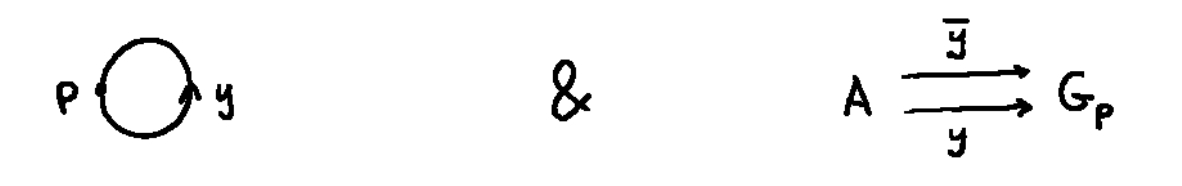
\includegraphics[width=0.5\linewidth]{sections/alicja/HNN loop and monomorphisms.jpeg}
    \caption{Graph $\Gamma$ and monomorphisms it comes with}
    \label{loopHNN}
\end{figure}

\begin{example}\cite[section I.5.1]{serre_trees_1980}\label{amalgexample}
    Let us now consider a graph of groups $\Gamma$ consisting of two vertices $p$, $q$ and a segment labelled by y between them, as shown in \ref{amalggraph}. As the maximal subtree of $\Gamma$ is the whole of $\Gamma$, the fundamental group $\pi_1(G,\Gamma,\Gamma)$ is $F(G,\Gamma)$ quotiented by the normal subgroup generated by $y$. Thus, we can think of it as being generated by groups $G_p$, $G_q$ subject to relation $a^y = a^{\overline{y}}$ for all $a \in G_y$. But $G_y$ is identified with a subgroup $A_1 \le G_q$ via $m_1 : a \mapsto a^y$ and with a subgroup $A_2 \le G_p$ via $m_2: a \mapsto a^{\overline{y}}$. Because those identifications are done via monomorphisms, this means that $A_1 \cong A_2$, via $\phi: A_1 \to A_2$, $l \mapsto m_1^{-1}(l) \mapsto m_2(m_1^{-1}(l))$ for all $l \in A_1$. Thus the presentation of $\pi_1(G,\Gamma,\Gamma) = \langle G_p,G_q \: | \: l = \phi(l), l \in A_1\rangle$, which is exactly $G_p\ast_{A_1}G_q \cong G_p \ast_{G_y}G_q$ (Compare this with a definition of amalgamated free product \ref{defnamalgamatedproduct}).
\end{example}



\begin{figure}[h]
    \centering
    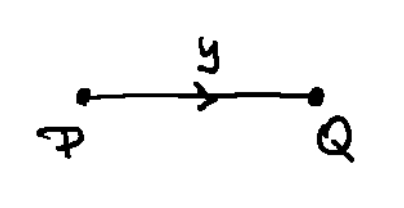
\includegraphics[scale = 0.14]{sections/alicja/Segment of groups.jpeg}
    \caption{Graph $\Gamma$ described in \ref{amalgexample}}
    \label{amalggraph}
\end{figure}

\begin{remark}
    One could now see why we needed to see both the graph of groups for a HNN extension and for an amalgamated free product. Each of those corresponds to a fundamental building block of a general graph of groups, namely a loop at a point or an edge.
\end{remark}

\begin{importantexample}[\ref{HNN graph} for BS groups] \label{BS graph} In this example we will use multiplicative notation when talking about $\Z = \langle b \rangle$. 

We let $Y$ be a graph with vertex group $G_p = \Z$, and edge group $G_y = m\Z$. We set the monomorphism $a \mapsto a^y$ to be $(b^m)^k \mapsto (b^m)^k$, and this identifies $m\Z$ with its copy living inside $\Z$. We let the other morphism be $\phi: m\Z \to \Z$, $(b^m)^k \mapsto (b^n)^k$. Note, that $\phi$ is actually mapping $m\Z$ into $n\Z$ inside $\Z$. Using that observation, the fundamental group of $Y$ is $\Z \ast _\phi$, which by \ref{BS as HNN} is the group $BS(m,n)$. Finally, note that $g_y$ mentioned in \ref{HNN graph} is equal to $t$ in this case.
\end{importantexample}

The next construction will be based on \cite[pages 23-24]{GoPaXi24}, cross-referenced with \cite{Wil} and \cite{BajoHNN}, where in the latter the less general case is discussed.

\begin{construction} \label{universalcover}
    Let $\mathbb{X} = (G,\Gamma)$ be a graph of groups, with underlying graph $\Gamma$ and fundamental group $\pi = \pi_1(G,\Gamma,T)$, where $T$ is a maximal tree of $\Gamma$.
    The Bass-Serre tree $\Tilde{X}$ of $\mathbb{X}$ is constructed as follows:
    \begin{itemize}
        \item it has vertices $V(\Tilde{X}) = \{\pi/G_x\:|\: x \in V(\Gamma)\}$, and
        \item its edges are $E(\Tilde{X}_+) = \{\pi/\phi(G_y) \: | \: y \in E(\Gamma_+)\}$, where
        \item for each $g\phi(G_y) \in E(\Tilde{X}_+)$, $i(g\phi(G_y)) = gG_{i(y)}$ and $t(g\phi(G_y)) = gg_yG_{t(y)}$.
    \end{itemize}
\end{construction}

Having stated the construction, two questions should come to mind, namely - why is this a connected graph and moreover, a tree. Instead of addressing those, we will see what this construction gives for $BS(m,n)$, and hopefully believe the resulting graph is indeed a tree.


\begin{importantexample}
    To construct the Bass-Serre tree of the Baumslag-Solitar group $BS(m,n) = \langle b,t \: | \: tb^mt^{-1} = b^n \rangle$, we will use its graph of groups $\mathbb{X}$, which was described in \ref{BS graph}. Recall that $\mathbb{X}$ is a loop, i.e. has only one vertex, with vertex group $G_x = \Z = \langle b\rangle$, and an edge attached to said vertex, with edge group $G_y = m\Z$. Thus, vertices of $\Tilde{X}$ are cosets $g\Z$, and edges are $g(\phi(m\Z)) = g(n\Z)$, with $g \in BS(m,n)$. Let us denote $H=n\Z$. Finally, for each edge $gH$, if we assume it is in $E(\Tilde{X}_+)$, $o(gH) = g\Z$ and $t(gH) = gt(n\Z)$.
    The resulting graph is depicted in \ref{BS tree}.
    The following are worth noting:
    \begin{enumerate}
        \item because of the relation $tb^mt^{-1} = b^n$, we get that $tb^m = b^nt$ and $b^mt^{-1} = t^{-1}b^n$. Thus $b^nt\Z = tb^m\Z = t\Z$ are all the same coset, and if $0 \le f <n$, then $b^ft\Z \neq t\Z$. This is because, if they were equal, it would mean that we have a relation $b^f = tb^lt^{-1}$ for some $l \in \Z$, which is not true. Similarly, $b^mt^{-1}\Z = t^{-1}b^n\Z = t^{-1}\Z$ and for all $0 \le f <m$, then $b^ft^{-1}\Z \neq t^{-1}\Z$.
        This explains why the described vertices appear as adjacent to the vertex labelled by $\Z$ in the figure.
        \item As $BS(m,n)$ acts on $\Tilde{X}$ by automorphisms, and above we saw that the coset $\Z$ corresponds to a vertex of valence $n+m$, all vertices will have that valence. 
    \end{enumerate}
\end{importantexample}

\begin{figure}[ht]
    \centering
    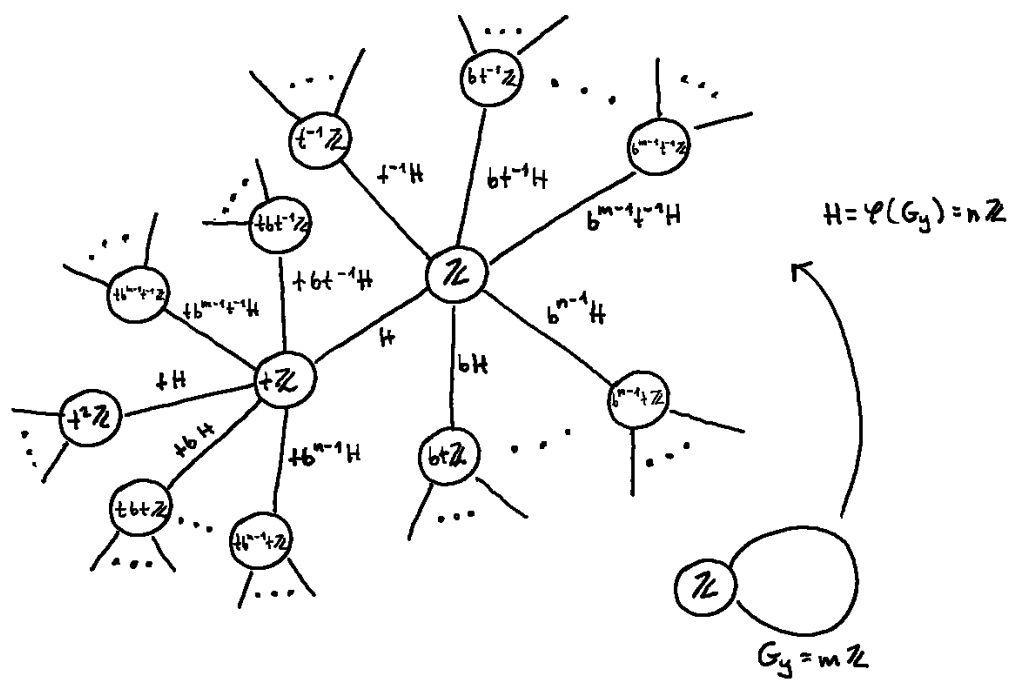
\includegraphics[scale = 0.38]{sections/alicja/Tree of BS(m,n) corrected.jpeg}
    \caption{Bass-Serre tree for $BS(m,n)$}
    \label{BS tree}
\end{figure}

We have discussed the graph with fundamental group $BS(m,n)$, as well as, the tree associated to it. We can now go on to generalise Baumslag-Solitar groups.

\subsection{Generalised Baumslag-Solitar (GBS) groups}
In the previous section we saw the connection between certain trees and graphs of groups. It should then come as no surprise that we can define our group in terms of one or the other. 
Depending on what properties of $GBS$ groups one wants to explore, one of the following definitions might be preferable.

\begin{definition}[\cite{For03}]
    A \emph{generalised Baumslag-Solitar tree} is a $G$-tree whose vertex and edge stabilisers are all infinite cyclic. The groups $G$ that arise this way are called \emph{generalised Baumslag-Solitar groups}.
\end{definition}

\begin{definition}[\cite{Le07}]\label{GBSgofg}
    A \emph{generalised Baumslag-Solitar group} $G$ is the fundamental group of a finite graph of groups $\Gamma$ whose vertex and edge groups are all infinite cyclic.
\end{definition}

Let us start by looking at some examples of $GBS$ groups.

\begin{example}
    As one would hope, Baumslag-Solitar groups $BS(m,n)$ are $GBS$ groups. One can see it using the definition \ref{GBSgofg} -  a graph with the fundamental group $BS(m,n)$ which we obtained in \ref{BS graph} has vertex and edge groups $\Z$ and $m\Z$, respectively.
\end{example}

\begin{example} 
    A torus knot group, $T(p,q) = \langle x,y | x^p = y^q \rangle$ where $p$,$q$ are distinct primes, is a $GBS$ group.

    This can be seen by considering the graph of groups from figure \ref{T(p,q) graph}, which by the discussion in \cite{Jo23} has $T(p,q)$ as its fundamental group.
\end{example}

\begin{figure}[h]
    \centering
    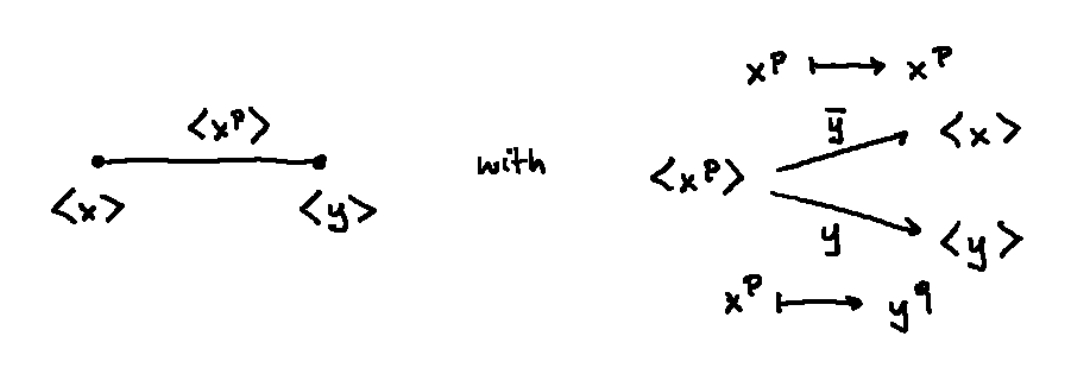
\includegraphics[width=0.5\linewidth]{sections/alicja/Graph for T(p,q).jpeg}
    \caption{Graph of groups for $\langle x \rangle \ast_{x^p = y^q} \langle y \rangle$ and morphisms it comes with} 
    \label{T(p,q) graph}
\end{figure}

Having seen the two examples which get quoted most often in the literature as first examples of $GBS$ groups, we can now consider a collection of results about this class of groups.

\subsubsection{Elementary $GBS$ groups} \label{labelledGBSgraph}
Firstly, note that, as $GBS$ graphs $\Gamma$ have all edge and vertex groups infinite cyclic, we can choose their generators. Then, the inclusion maps of edge groups into vertex groups become multiplications by non-zero integers. Thus, we can endow an oriented edge $e$ with a label $\lambda_e \in \Z \setminus \{0\}$ describing the inclusion of $G_e$ into $G_{i(e)}$. A pair of opposite edges $\epsilon = (e,\overline{e})$ is a non-oriented edge, and it can be endowed with a label $(\lambda_e,\lambda_{\overline{e}})$. Note, that this construction can be applied to both loops and segments of a graph $\Gamma$.

In \cite{Le07} Levitt makes the following distinction.

\begin{remark} \label{elemlinegbs}
    The elementary $GBS$ groups $G$, with $\Gamma$ being a graph of groups with $\pi_1(\Gamma) = G$ are:
    \begin{itemize}
        \item $\Z$ with $\Gamma$ = point,
        \item $\Z^2$ with $\Gamma$ = $(1,1)$-loop,
        \item Klein bottle group $K = \langle x,t \: | \: txt^{-1} = x^{-1} \rangle = \langle a,b \: | \: a^2 = b^2\rangle$ with either $\Gamma$ = $(1,-1)$-loop or $(2,2)$-segment.
    \end{itemize}
    The feature that the above have in common is that the Bass-Serre tree $T$ associated to each of them is either a point or a line. Moreover, they are the only graphs for which that holds.
\end{remark}

\begin{figure}[h]
    \centering
    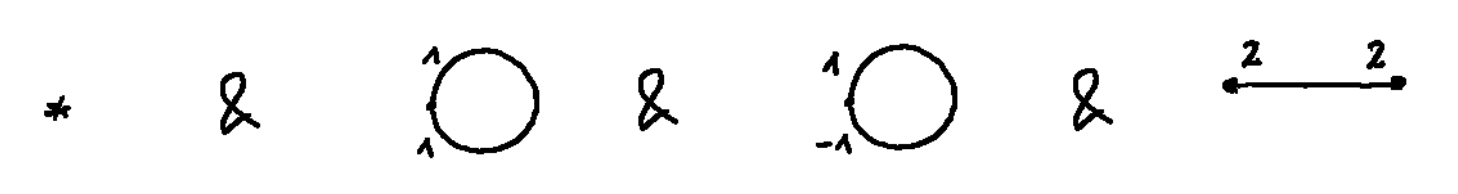
\includegraphics[scale = 0.15]{sections/alicja/Elementary graphs.jpeg}
    \caption{Graphs with elementary $GBS$ fundamental groups}
    \label{elementarygraphs}
\end{figure}

\subsubsection{Properties of $GBS$ groups developed in \cite{For03}}
\label{JSJ} % Hello, I hope you don't mind me labelling this so I can refer to your discussion on JSJ decomposition :) -Talia
This paper concerns JSJ decompositions and their uniqueness for finitely presented groups, and uses $GBS$ trees as examples. Thus, the paper reviews some properties of $GBS$ groups.

Firstly let us remark on JSJ decompositions and then we will proceed to state some definitions for the situation when we have any $G$-tree.

\begin{remark}\cite{GuLe17}
    JSJ decompositions first appeared in the context of 3-dimensional topology of manifolds. For a group $G$ its \emph{JSJ decomposition} over a given family of its subgroups $\mathcal{A}$ is an $\mathcal{A}$-tree $T$ satisfying certain properties. By an $\mathcal{A}$-tree we mean a $G$-tree $T$ whose edge stabilisers are in $\mathcal{A}$. It is important to note, that JSJ decompositions do not always exist and if they do, they are not unique.

    The aim of \cite{For03} is to use two $GBS$ trees as example of JSJ decompositions of a finitely presented group $G$ which are not related by conjugation, conjugation of edge-inclusions, and slide moves. That gives a negative answer to the question of Rips and Sela.
\end{remark}

\begin{definition}
    Let $T$ be a $G$-tree. An element $\gamma \in G$ is called \emph{elliptic} if it fixes a vertex of $T$. Otherwise $\gamma$ is said to be \emph{hyperbolic}.
    
    Elements $\gamma,\delta \in G$ are defined to be \emph{commensurable} if there exist $m,n \in \Z\setminus \{0\}$ such that $\gamma^m = \delta^n$. The \emph{commensurator} of $\gamma$ is the set of all $\delta \in G$ such that $\delta\gamma\delta^{-1}$ and $\gamma$ are commensurable. We denote it as $Comm(\gamma)$.
\end{definition}

\begin{remark}
    As shown in \cite[Proposition 24]{serre_trees_1980} if $\gamma$ is hyperbolic, then there is a $\gamma$-invariant path (or line) in $T$, on which $\gamma$ acts by translation. We call this path an \emph{axis} of $\gamma$.
\end{remark}

\begin{lemma}[{\cite[2.5]{For03}, \cite[2.1]{Le07} combined}]\label{ellipticcomm}
    Let $T$ be a $G$-tree. If $\gamma \in G$ is hyperbolic then $Comm(\gamma)$ stabilises its axis. If additionally $T$ is a $GBS$ tree with $G$ non-elementary, then any two nontrivial elliptic elements $\gamma,\delta$ are commensurable, and the commensurator for an elliptic element $\gamma$ is the whole of $G$.
\end{lemma}

\begin{remark}
    Assuming that $T$ is a $GBS$ tree with non-elementary $G$ actually grants us something more. According to \cite[2.1]{Le07}, in that situation, an element $\gamma \in G$ is elliptic if and only if its commensurator equals $G$. This is because, if $\gamma$ is hyperbolic, then its axis is invariant under $Comm(\gamma)$. Thus, $G \neq Comm(\gamma)$, as $T$ is not a point or a line. The latter comes from the feature that we pointed out about the graphs of elementary groups in \ref{elemlinegbs}.
\end{remark}

We are also able to state a lemma concerning subgroups of a $GBS$ group.

\begin{lemma}
    Let $T$ be a $GBS$ tree with group $G$. Every subgroup $H$ of $G$ is either a generalised Baumslag-Solitar group or a free group (and not both, unless $G = \Z$). If $H$ is free and non-abelian, then every non-trivial element of $H$ is hyperbolic.
\end{lemma}

The final result of this part of the section is below to showcase some other interesting properties of $GBS$ groups. Some concepts that appear in it will not be explored in this chapter or this project at all, but we will provide on some references for an interested reader.

\begin{lemma}
    Let $T$ be a $GBS$ tree with group $G \ncong \Z$. Then:
   \begin{enumerate}
        \item G is not free;
        \item G is torsion free and has cohomological dimension 2;
        \item G has one end, if it is finitely generated;
        \item T contains a $G$-invariant line if and only if $G$ is isomorphic to $\Z \times \Z$ or the Klein bottle group.
    \end{enumerate}  
\end{lemma}

\begin{remark}
    The following comments are worth making about the above lemma:
    \begin{itemize}
        \item Recall, that an infinite group is said to be torsion free if it contains no finite order elements.
        \item As the cohomological dimension will not be explored in this project, one of the references the reader could look at is \cite{Br}. If familiar with the concept the paper of P. Kropholler \cite[Theorem C]{Kr90} provides an interesting result. It states that a non-cyclic group belongs to a certain class of finitely generated groups of cohomological dimension 2 if and only if it is a fundamental group of a finite graph of infinite cyclic group. The latter is exactly a non-cyclic $GBS$ group, in light of definition \ref{GBSgofg}.
        \item The reader can explore the concept of ends in Section \ref{Ends of groups}.
    \end{itemize}
\end{remark}

We will now go on to state a result which tells us information about all generalised Baumslag-Solitar groups.

\subsubsection{Classification of $GBS$ graphs}

\begin{remark}
    Note, that sometimes $GBS$ graphs are called \emph{graphs of $\Z$s}. This again points at how $GBS$ groups generalise Baumslag-Solitar groups, as $BS$ groups are precisely the HNN extensions of $\Z$.
\end{remark}

The following theorem of Whyte classifies graphs of $\Z$, thus by the above remark, $GBS$ graphs.

\begin{theorem}\cite[Theorem 0.1]{WH01}\label{classgrZ}
    If $\Gamma$ is a graph of $\Z$s and $G= \pi_1(\Gamma)$ then exactly one of the following is true:
    \begin{enumerate}
        \item $G$ contains a subgroup of finite index of the form $F_n \times \Z$, where $F_n$ is the free group on $n$ generators.
        \item $G = BS(1,n)$ for some $n > 1$.
        \item $G$ is quasi-isometric to $BS(2,3)$.
    \end{enumerate}
\end{theorem}

\begin{corollary}
    All the groups $BS(m,n)$ with $1 < m <n$ are quasi-isometric to each other.
\end{corollary}

\begin{remark}
    Recall that a map $f: X \to Y$ between two metric spaces is called a quasi-isometry if there exist constants $\lambda \ge 1$, $c \ge 0$ and $K$ such that:
    \begin{enumerate}
        \item $\frac{1}{\lambda}d_X(x,x') - c \le d_Y(f(x),f(x')) \le \lambda d_X(x,x') + c$ (q-i embedding), and
        \item $\forall y \in Y$ $ \exists x \in X$ with $d(y,f(x)) \le K$ (quasi-surjectivity).
    \end{enumerate}
    We can think of a finitely generated group $G$ as a metric space, as given a generating set $S$ of $G$, we can consider the word metric $d_S$. Recall, that $d_S(g,h) = l_S(g^{-1}h) = \{length \; of \; a\;shortest \; word \; representing \; g^{-1}h \; in \; S\cup S^{-1} \}$. It is a fact that if $S$, $T$ are both finite generating sets for $G$, then $(G,d_S)$ and $(G,d_T)$ are quasi-isometric. We say that two finitely generated groups $G$, $H$ are \emph{quasi-isometric} if there exists a quasi-isometry $f: (G,d_S) \to (H,d_T)$ where $S$, $T$ are generating sets of $G$, $H$, respectively.
\end{remark}

In the sketch below we will be following an outline that was provided in \cite{WH01}.

\begin{proof}[Idea of proof of \ref{classgrZ}]
    Let us start by letting $G$ be the fundamental group of a graph of groups $\Gamma$, $T$ a Bass-Serre tree for $G$. The main ideas of the argument are:
    \begin{itemize}
        \item We can construct $X_G$ which in appropriate sense reflects the geometry of $G$, and on which $G$ acts nicely.
        \item The constructed $X_G$ is a contractible $2$-complex, which topologically is a product $T \times \R$. Metrically, it differs from the product metric by $v \times \R$ getting scaled by a fitting warping function $T \to \R^+$.
        \item Due to the construction, the warping function depends on height change between vertices. Said height change can be seen as quantitative analogue of orientation.
        \item The classification of graphs of $\Z$s reduces to classifying coarsely oriented trees. This is by showing that being given a quasi-isometry between the graphs there is a quasi-isoetry coarsely respecting orientation between trees, and vice versa when given a coarsely orientation preserving quasi-isometry between Bass-Serre trees.
        \item Due to caring about coarsely orientation preserving quasi-isometries, we can consider a special type of trees and develop their classification.
        \item The final quasi-isometries are by considering lines of ``constant slope'' and building quasi-isometries line by line.
    \end{itemize}
The above are sufficient to classify graphs of $\Z$s up to quasi-isometry.
\end{proof}


\subsubsection{Quotients and subgroups of $GBS$ groups} In this final subsection we will follow the work \cite{Le15} of Levitt. That reference contains many interesting results, and thus we will only state and comment on a few of them. If any of the statements pique readers interest, they are encouraged to find their proofs and context in the paper.

\begin{lemma}\cite[Lemma 2.1]{Le15}
    Any 2-generated $GBS$ group $G$ is a quotient of some $BS(m,n)$.
\end{lemma}

\begin{proof}[Idea of proof]
 This lemma follows, if we show that there is a generating pair $(a,t)$ for $G$, with $a$ elliptic. We will take that on faith and proceed, an interested reader can take a look at the comments in the paper. Thus, assume we have such pair. Then as $a$ is elliptic, by \ref{ellipticcomm}, its commensurator is the whole of $G$, so in particular $tat^{-1}$ is in it. Then $(a,t)$ satisfy the relation $ta^mt^{-1} = (tat^{-1})^m = a^n$ for some non-zero integers $m,n$. Therefore, $G$ is a quotient of $BS(m,n)$ by any other occurring relations.
\end{proof}

\begin{definition}
    At the beginning of subsection \ref{labelledGBSgraph} we introduced a way of labelling a $GBS$ graph of groups $\Gamma$. We call $\Gamma$ \emph{reduced} if any edge $e$ such that $\lambda_e \in \{-1,1\}$ is a loop.
\end{definition}

\begin{remark}
    Any labelled graph can be reduced by a sequence of elementary collapses, which do not change $G$. If we have a segment in our graph it corresponds to an amalgamated free product. Let us see what happens if one of its ends has label 1, as on the figure \ref{collapsingedge} (note that vertex groups are marked with capital letters, edge lables with greek letters). Then as described in \cite{For06}, such edge can be shrunk to the point, which corresponds to replacing $A \ast_C C$ with $A$. 
\end{remark}

\begin{figure}[h]
    \centering
    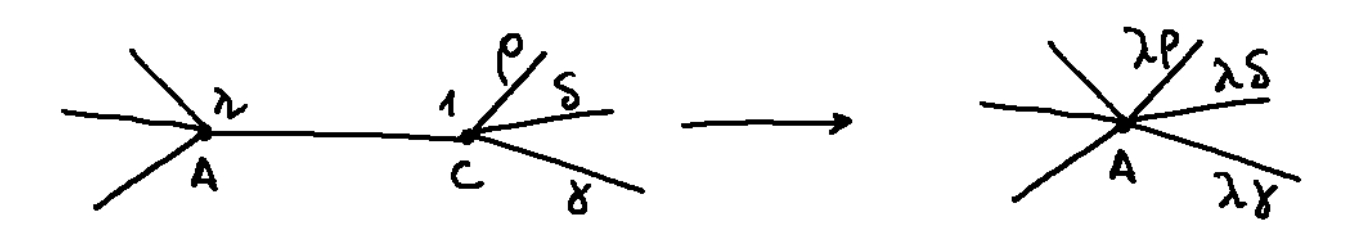
\includegraphics[scale=0.15]{sections/alicja/collapse move.jpeg}
    \caption{Collapsing an edge with one of the labels being 1}
    \label{collapsingedge}
\end{figure}

\begin{remark}
    There are other moves that we can perform on a graph of groups $\Gamma$, and they are described in eg. \cite{For06}.
\end{remark}

\begin{lemma}\cite[Lemma 2.8]{Le15}
    If a $GBS$ group $G$ is $2$-generated and is not a solvable $BS(1,n)$, it may be represented by a labelled graph with no label equal to $1$ or $-1$.
\end{lemma}

There is more that we can say about a $GBS$ graph if we make other assumptions.

\begin{proposition}\cite[Proposition 5.1]{Le15}
    Let $\Gamma$ be a reduced labelled graph representing a $GBS$ group $G$ which is a quotient of $BS(m,n)$.
    \begin{enumerate}
        \item There is a bound, depending only on $m$ and $n$, for the number of edges of $\Gamma$.
        \item If $m \neq n$ and $G$ is not the Klein bottle group $K$, every prime $p$ dividing a label of $\Gamma$ must divide $mn$.
    \end{enumerate}
\end{proposition}

\begin{remark}
    The proof of this proposition follows from using a result \cite[Theorem 4.1]{Le15}, which tells us information about labels of a graph $\Gamma$ of a $2$-generated $GBS$ group depending on the structure of $\Gamma$. The possible graphs in that case look either like segments, or like lollipops and those two cases are considered in a proof of the above.
\end{remark}

A corollary of \cite[Proposition 5.6]{Le15} tells us how to read off information about quotients from the $GBS$ graph.

\begin{corollary}\cite[Corollary 5.7]{Le15}
    If $BS(m,n)$ has a $GBS$ quotient $G \neq K$ represented by a labelled graph $\Gamma$ with no label $\{-1,1\}$ such that $\Gamma$ is not homeomorphic to a circle, then $BS(m,n)$ has infinitely many non-isomorphic $GBS$ quotients.
\end{corollary}

\begin{remark}
    The other results of the paper concern maps between $GBS$ groups, conditions for when one Baumslag-Solitar group embeds in the other, results about subgroups of $BS(n,n)$ and much more.
\end{remark}

Both \cite{Le15} and \cite{WH01} obtain results about Baumslag-Solitar groups by using $GBS$ groups. It is thus important to note, that $GBS$ groups can be studied both because they are interesting groups to consider and because they provide a way to learn more about Baumslag-Solitar groups.


\subsection{Concluding remarks}
This section is not an exhaustive account of either all the properties or work on (generalised) Baumslag-Solitar groups. Thus, it seems fitting to mention some other properties and papers which have not been discussed in the course of our exploration.
\begin{enumerate}
    \item An interesting question is that of growth of Baumslag-Solitar groups. A starting reference could be \cite{Ha00} where definitions of growth and some references to the current results are provided. There also newer papers on the topic, e.g. \cite{SaSh18} or \cite{FrKnSch11}.
    \item Despite $BS(m,n)$ being amenable if and only if $|m| = 1$ or $|n| = 1$ \cite{CaGaMaSt24}, considering weaker forms of amenability for Baumslag-Solitar is still a worthwhile endevour. See for example \cite{CoVa15}.
    \item As we have seen in \ref{BSisom}, the isomorphism problem for Baumslag-Solitar groups has a straightforward answer. This is however not the case for the $GBS$ groups, and the account of that can be found in \cite{ClFo08}.
\end{enumerate}

With the above list we finish the dive into Baumslag-Solitar groups and proceed to the next parts of the report.



\section{Complexes of groups}
\todo[color=olive]{Hello Sean, it's Ala.
	Feel free to ignore any suggestions I make - I chose a different colour so its clear which are my notes.
	I also corrected any grammar and punctuation that I noticed, but I might have not caught everything.}
In this section we will introduce the construction of \emph{complexes of groups}, largely due to Haefliger \cite{haefliger_complexes_1991}.
This generalises the construction of graphs of groups due to Bass and Serre, discussed in REF.
\todo[color=olive]{Remember to add the reference instead of "REF"}
A related construction of \emph{triangles of groups} was studied by Gersten and Stallings \cite{stallings_nonpositively_1991} and complexes of groups were studied in two dimensions, independently of Haefliger, by Corson \cite{corson_complexes_1992}.
The exposition here largely follows \cite[Chapter 3.\textrm{\ensuremath{\calc}}]{BrHa11}, with some modification to notation and with some elements explored in more detail.

The construction of graphs of groups arose by abstracting emergent features of group actions on trees.
Analogously, to define complexes of groups, we will consider certain group actions on geometric complexes associated to so-called \emph{small categories without loops}.
However, unlike with graphs of groups, not every complex of groups can be realised as a quotient of group action on a complex.

\subsection{Small categories without loops}

We will first recall the standard construction of the geometric realisation $\abs{P}$ of a poset $P$.
Given a poset $P$, a chain $C \subseteq P$ is a totally ordered subposet, i.e.~either $x \leq y$ or  $y \leq x$ for all  $x,y \in C$.
We say $C$ is an $n$--chain if $n=\abs{C}-1$.
We denote the standard $k$--simplex as $\Delta^k$, where
\[
	\Delta^k \coloneq \Set{(x_0,\ldots, x_k) \in \R^{k+1} \given x_i \geq 0 \; \forall i \text{ and } x_0 + \cdots + x_k =1}
	.\]

To construct $\abs{P}$, we first associate to each $n$--chain in $P$, an $n$--simplex $\Delta_{C}$.
The elements of $C$ correspond to the vertices of $\Delta_{C}$.
Such a $\Delta_C$, and all of its faces, are canonically oriented due to the ordering in $P$.
Using this orientation, we glue simplices corresponding to subchains to a face of the higher dimensional simplex, which corresponds to the superchain.
Specifically, let $C_1 \subset C_2$ be chains, with $C_1$ an $n$--chain.
Let $f$ denote the orientation preserving isometry from (the closed) $\Delta_{C_1}$ to the relevant (closed) $n$--dimensional face of $\Delta_{C_2}$.
We then glue $\Delta_{C_1}$ to $\Delta_{C_2}$ using  $f$.
Taking $\sim$ to be the transitive closure of the relation defined by all such $f$, for all chains and subchains of  $P$, we then have
\[
	\abs{P} \coloneq \left(\;\bigsqcup_{\substack{ C \subseteq P \\ \text{chain}}} \Delta_C \right)/\sim
	.\]

See \cref{fig:example_poset_complex} for an example, where $\abs{P}$ is three solid tetrahedrons.
Two tetrahedrons, on the left half of the picture, share a face, and all three tetrahedrons share an edge, which is vertical and centred in the picture.

% filled small circle
\tikzstyle{FSC}=[circle, draw=black!50,fill=black!20,thick, inner sep=0pt,minimum size=1.5mm]
\tikzstyle{light}=[black!22!white]

\begin{figure}
	\centering
	\begin{tikzpicture}
		\tikzstyle{every label}=[font=\footnotesize]
		\tikzstyle{every node}=[font=\footnotesize]
		\node[FSC] (base)		at (0,0)				[label=below:$\emptyset$]			{};
		\node[FSC] (bottom left)	at ($(base) + (-0.8,1) $)   		[label={[label distance=-0.1cm]200:$\{1\}$}]    {};
		\node[FSC] (bottom right)	at ($(bottom left) + (1.6,0)$)  	[label={[label distance=-0.1cm]300:$\{2\}$}]    {};
		\node[FSC] (top left)		at ($(bottom left) + (-1.1,1)$)    	[label=left:{$\{1,4\}$}]          		{};
		\node[FSC] (top middle)    	at ($(base) + (0,2)$)  			[label=right:{$\{1,3\}$}]			{};
		\node[FSC] (top right)    	at ($(bottom right) + (1.1,1)$)  	[label=right:{$\{2,3\}$}]          		{};
		\node[FSC] (top)          	at ($(base) + (0,3)$)    		[label=above:{$\{1,2,3,4\}$}]			{};

		\draw (base) 		to 	node[auto] 		{} 	(bottom left);
		\draw (base) 		to 	node[auto, swap] 	{} 	(bottom right);
		\draw (bottom left)		to 	node[auto] 		{} 	(top left);
		\draw (bottom left)		to 	node[auto] 		{} 	(top middle);
		\draw (top middle)		to 	node[auto]		{}	(top);
		\draw (bottom right)		to 	node[auto, swap] 	{} 	(top right);
		\draw (top left)		to 	node[auto] 		{} 	(top);
		\draw (top right)		to 	node[auto, swap] 	{} 	(top);
	\end{tikzpicture}
	\hspace{1cm}
	\begin{tikzpicture}[baseline=-18pt]
		\node[FSC] (base)          	at (0,0)					{};
		\node[FSC] (bottom left)	at ($(base) + (-0.9,1) $)			{};
		\node[FSC] (bottom right)	at ($(bottom left) + (1.6,0)$)  		{};
		\node[FSC] (top left)		at ($(bottom left) + (-1.1,0.5)$)		{};
		\node[FSC] (top middle)    	at ($(base) + (-0.22,1.15)$)			{};
		\node[FSC] (top right)    	at ($(bottom right) + (1.1,0.5)$)		{};
		\node[FSC] (top)          	at ($(base) + (0,3)$)    			{};

		\draw (base) 			to					(bottom left);
		\draw (base) 			to 	  				(bottom right);
		\draw (bottom left)		to 	 				(top left);
		\draw (bottom left)		to 	 				(top middle);
		\draw (top middle) 		to 					(top);
		\draw (bottom right)	 	to 	  				(top right);
		\draw (top left) 		to 	 				(top);
		\draw (top right) 		to 	  				(top);


		\begin{pgfonlayer}{background}
			\draw[light] (base) 			to 	 				(top middle);
			\draw[light] (base) 			to 	  				(top);
			\draw[light] (base) 			to 	 				(top left);
			\draw[light] (base) 			to 	 				(top right);
			\draw[light] (bottom left) 	to 					(top);
			\draw[light] (bottom right) 	to 	  				(top);
		\end{pgfonlayer}
	\end{tikzpicture}
	\caption{The diagram of a poset where $\leq$ is $\subseteq$ (left) and a picture of the corresponding complex $\abs{P}$ (right) with the original poset highlighted in black.}
	\label{fig:example_poset_complex}
\end{figure}

Posets, and the construction $\abs{P}$, give a combinatorial description of certain simplicial complexes.
However, not all complexes can be realised by this construction.
For example, consider $S^1$ realised as two edges connected at their ends.
This limitation is linked to the following.

\begin{observation}
	All the information of a poset $P$ is encoded exactly by the following category $\calc$:
	The objects of  $\calc$ are the elements of  $P$, and there is a morphism  $x \to y$ in  $\calc$ exactly when  $x \leq y$ in $P$.
	The category $\calc$ is \emph{thin}, meaning that for all  $x,y \in \ob(\calc)$, there is at most one morphism  $x \to y$.
\end{observation}
Bearing this in mind, with the aim of being able to construct $S^1$ in a combinatorial way, we give the following definition.
We say a category $\calc$ is small if the collection of morphisms of $\calc$ fits in to a set.

\begin{definition}
	A small category without loops (abbreviated scwol), is a small category $\calx$ such that for all composable morphisms $x_1 \to x_2 \to \cdots \to x_n$, if $x_1=x_n$, then $x_1=x_i$ for all $i$, and each morphism is $\id_{x_1}$.
	\label{def:scwol}
\end{definition}

Note that this definition means that no two distinct objects are isomorphic.
It also means that the only morphism $x \to x$ is $\id_x$.
Conversely, if a small category satisfies both of these properties, then it is a scwol.

With geometry in mind, we call the objects of a scwol $\calx$ \emph{vertices} and denote the set of vertices by $V(\calx)$.
We call the non--identity morphisms of  $\calx$ \emph{edges} and denote the set of edges by $E(\calx)$.
Given some $a \in E(\calx)$, we denote the initial (source) and terminal (target) vertices by $i(a)$ and $t(a)$ respectively.
If two edges $b$ and $a$ satisfy $t(b)=i(a)$, then we say that $a$ and $b$ are composable and denote their composition $ab$, which is necessarily another edge in $E(\calx)$.
We have that $i(ab) = i(b)$ and $t(ab) = t(a)$.
We now work to construct a geometric realisation $\abs{\calx}$ of a scwol $\calx$, such that if $\calx$ is thin, then $\abs{\calx}$ matches the geometric realisation when considering $\calx$ as a poset.

Let $E^{(n)}(\calx)$ denote the set of all $n$--tuples of composable edges in $\calx$,
i.e.~if $(a_1, a_2, \ldots, a_n) \in E^{(n)}(\calx)$, then
\[
	\begin{tikzcd}
		x_1 \ar[r, "a_1"] & x_2 \ar[r, "a_2"] & {} \ar[r, phantom, "\cdots"] & {} \ar[r, "a_n"] & x_{n+1}
	\end{tikzcd}
\]
is a composable set of edges in $\calx$.
Since all the $a_i$ are in $E(\calx)$, none are identity morphisms.
By convention, $E^{(0)}(\calx) = V(\calx)$.
We define the following maps, $\partial_i \colon E^{(n)}(\calx) \to E^{(n-1)}(\calx)$ on composable tuples, where
\begin{align*}
	\partial_0(a_1,\ldots,a_n) & = (a_2,\ldots,a_n)                                          \\
	\partial_i(a_1,\ldots,a_n) & = (a_1, \ldots, a_ia_{i+1}, \ldots, a_n) \quad 1 \leq i < k \\
	\partial_n(a_1,\ldots,a_n) & = (a_1, \ldots, a_{n-1})
	.\end{align*}

\todo[color=olive]{It seems like $\partial_i$ has too many coordinates as outputs -  shouldn't it be $(a_1, \ldots, a_{i-1},a_{i+1},\ldots,a_n$? Also, shouldn't $i$ be in range $1 \le i <n$?}
We define $\partial_0(a)=i(a)$, and $\partial_1(a)=t(a)$.
We also define maps, $d_i \colon \Delta^{k-1} \to \Delta^k$ on simplices, where
\[
	d_i(t_0, \ldots, t_{k-1}) = (t_0, \ldots, t_{i-1}, 0, t_i, \ldots, t_{k-1}) \quad 0 \leq i < k
	.\]

\begin{definition}
	Given a scwol $\calx$, the geometric realisation, $\abs{\calx}$ is a simplicial complex defined as
	\[
		\abs{\calx} \coloneq \bigsqcup_k \left( \Delta^k \times E^{(k)}(\calx) \right) / \sim
		.\]
	Where $\sim$ is the transitive closure of the relations
	\[
		(d_i(x),t) \sim (x, \partial_i(t))
	\]
	across all tuples $t \in E^{(k)}(\calx)$.
	\label{def:geometric_realisation_of_scwol}
\end{definition}
In this definition, we had to take more care than with the geometric realisation of a poset.
This is because, in a poset, a composable tuple is completely determined by its vertices (the chain), so the combinatorial face maps always corresponded to taking subsets of those vertices.
But in a scwol, we need to account for potentially multiple edges between two vertices, so we must enumerate simplices using edges, rather than vertices.

For those interested, the above construction of $\abs{\calx}$ corresponds to the standard geometric realisation of the nerve (which corresponds to the union of all of our $E^{(k)}(\calx)$) of $\calx$.
See \cite{goerss_simplicial_2009}.

Given a scwol $\calx$, the dimension of  $\calx $ is the dimension of $\abs{\calx}$, this is the largest  $k$ such that  $E^{(k)}(\calx) \neq \emptyset$.

\begin{example}
	The following scwol has geometric realisation $S^1$, constructed by identifying the ends of two 1--simplices.
	\begin{center}
		\begin{tikzpicture}
			\tikzstyle{every label}=[font=\footnotesize]
			\tikzstyle{every node}=[font=\footnotesize]
			\node[FSC] (base)	at (0,0)	{};
			\node[FSC] (top)	at (0,1)	{};
			\draw[arrow_me=stealth, bend left=90] (base) to (top);
			\draw[arrow_me=stealth, bend right=90] (base) to (top);
		\end{tikzpicture}
	\end{center}
\end{example}

\begin{example}
	Any polygon can be realised as the geometric realisation of a scwol $\calx$ in the following way:
	Consider the polygon as a polygonal complex.
	Make a vertex for at the centre of each polygon in the complex.
	\todo[color=olive]{What is "for" doing in this sentence?}
	There is an edge from centres of polygons to centres of faces of that polygon.
	The below picture shows the scwol from this construction applied to a square.
	\begin{center}
		\begin{tikzpicture}
			\def\sqsize{2}
			\tikzstyle{every label}=[font=\footnotesize]
			\tikzstyle{every node}=[font=\footnotesize]
			\node[FSC] (bl)	at (0,0)	{};
			\node[FSC] (br)	at ($(bl)+(\sqsize,0)$)	{};
			\node[FSC] (tl)	at ($(bl)+(0,\sqsize)$)	{};
			\node[FSC] (tr)	at ($(tl)+(\sqsize,0)$)	{};

			\node[FSC] (mblbr) at ($(bl)!0.5!(br)$) {};
			\node[FSC] (mbltl) at ($(bl)!0.5!(tl)$) {};
			\node[FSC] (mbrtr) at ($(br)!0.5!(tr)$) {};
			\node[FSC] (mtltr) at ($(tl)!0.5!(tr)$) {};

			\node[FSC] (center) at ($(bl)!0.5!(tr)$) {};

			\draw[arrow_me=stealth] (center) to (bl);
			\draw[arrow_me=stealth] (center) to (br);
			\draw[arrow_me=stealth] (center) to (tl);
			\draw[arrow_me=stealth] (center) to (tr);

			\draw[arrow_me=stealth] (center) to (mblbr);
			\draw[arrow_me=stealth] (center) to (mbltl);
			\draw[arrow_me=stealth] (center) to (mtltr);
			\draw[arrow_me=stealth] (center) to (mbrtr);

			\draw[arrow_me=stealth] (mblbr) to (bl);
			\draw[arrow_me=stealth] (mblbr) to (br);
			\draw[arrow_me=stealth] (mbltl) to (bl);
			\draw[arrow_me=stealth] (mbltl) to (tl);
			\draw[arrow_me=stealth] (mbrtr) to (br);
			\draw[arrow_me=stealth] (mbrtr) to (tr);
			\draw[arrow_me=stealth] (mtltr) to (tl);
			\draw[arrow_me=stealth] (mtltr) to (tr);
		\end{tikzpicture}
	\end{center}
	\label{eg:scwol_for_square}
\end{example}

\begin{example}
	Following the same procedure as the previous example, the scwol associated to the complete graph on three vertices is given below.
	\begin{center}
		\begin{tikzpicture}
			\def\trisize{1.5}
			\tikzstyle{every label}=[font=\footnotesize]
			\tikzstyle{every node}=[font=\footnotesize]

			\node[FSC] (bl)	at (0,0)	{};
			\node[FSC] (br)	at ($(bl)+(\trisize,0)$)	{};
			\node[FSC] (top) at ($(bl)+(0.5*\trisize,0.833*\trisize)$)	{};

			\node[FSC] (mblbr) at ($(bl)!0.5!(br)$) {};
			\node[FSC] (mblt) at ($(bl)!0.5!(top)$) {};
			\node[FSC] (mbrt) at ($(br)!0.5!(top)$) {};

			\draw[arrow_me=stealth] (mblbr) to (bl);
			\draw[arrow_me=stealth] (mblbr) to (br);
			\draw[arrow_me=stealth] (mblt) to (bl);
			\draw[arrow_me=stealth] (mblt) to (top);
			\draw[arrow_me=stealth] (mbrt) to (br);
			\draw[arrow_me=stealth] (mbrt) to (top);
		\end{tikzpicture}
	\end{center}
	\label{eg:K3_scwol}
\end{example}

\todo[color=olive]{A moral question: do we actually need scwols for the above example, i.e.
	the triangle? }

\begin{definition}
	Morphisms of scwols are exactly functors $F \colon \calx \to \caly$ where the source and target categories are scwols.
	We say that a morphism of scwols $F \colon \calx \to \caly$ is non-degenerate if $F$ maps $E(\calx)$ to  $E(\caly)$, and for all $v \in V(\calx)$, the restriction of  $F$ to $\Set{a \in E(\calx) \given i(a) = v}$ is a bijection on that set of edges.
\end{definition}


The requirement that $E(\calx)$ maps to $E(\caly)$ means that non-identity morphisms must be mapped to non-identity morphisms.
A morphism of scwols $F$ induces a map on the geometric realisations, we denote this $\abs{F}$.
This acts on each simplex $\Delta$ by the linear map determined by the image of the vertices of $\Delta$.
Non-degenerate maps are important because they do not reduce the length of compositions of non-identity maps, thus they preserve dimension.
The importance of the second condition is that if a group acts by non-degenerate morphisms, then the stabiliser of $i(a)$ is contained in the stabiliser of $a$, which is contained in the stabiliser of $t(a)$ by virtue of $F$  being a functor.
In this way, this condition guarantees that stabilisers respect the category structure.
The importance of this will become apparent when we define complexes of groups.

(Non-degenerate) automorphisms of a scwols are (non-degenerate) invertible morphisms $F \colon \calx \to \calx$.

\begin{definition}
	An action of a group $G$ on a scwol $\calx$ is a homomorphism from $G$ to the group of non-degenerate automorphisms of $\calx$ such that the following two conditions are met.
	\begin{enumerate}
		\item For all $a \in E(\calx)$ and $g \in G$, we have  $g \cdot i(a) \neq t(a)$.
		\item For all $a \in E(\calx)$ and $g \in G$, if  $g\cdot i(a)=i(a)$, then  $g\cdot a = a$.
	\end{enumerate}
	\label{def:action_of_groups_on_scwols}
\end{definition}
\todo{compare this def to that of actions without inversions in graphs of groups}

If $\calx$ is finite dimensional, then the first condition is guaranteed.
For example, in the following scwol, if $\sigma$ was mapped to  $\tau$, then $\tau$ is mapped to $\mu$ and there is nowhere for $a$ to map to.

\begin{center}
	\begin{tikzpicture}
		\def\size{0.9}
		\tikzstyle{every label}=[font=\footnotesize]
		\tikzstyle{every node}=[font=\footnotesize]

		\node[FSC, label=below:{$\sigma$}] (l) at (0,0)		{};
		\node[FSC, label=below:{$\tau$}] (m) at ($(l)+(\size,0)$)	{};
		\node[FSC, label=below:{$\mu$}] (r) at ($(m)+(\size,0)$)	{};

		\draw[arrow_me=stealth] (l) to node[below] {$b$} (m);
		\draw[arrow_me=stealth] (m) to node[below] {$a$} (r);
		\draw[arrow_me=stealth, bend left=90] (l) to node[above] {$ab$} (r);
	\end{tikzpicture}
\end{center}

However, if we consider the action of the group $\Z$ on the poset $\Z$, we see that  the first condition is not vacuous.

For each $g \in G$, denote the induced action on  $\abs{\calx}$ as $\abs{g}$.
The second condition means that if for some $\sigma \in V(\calx)$, we have $g \cdot \sigma = \sigma$, then $\abs{g}$ fixes pointwise any $k$-simplex corresponding to a composable tuple $(a_1,  \ldots, a_k)$ with $i(a_1)=\sigma$.
This in particular implies that if $\abs{g}$ fixes a simplex setwise, then it also fixes it pointwise.
This is important because we want to be able to quotient by this group action and for the quotient map to be simplicial on $\abs{\calx}$.
Note that these restrictions mean that many group actions that geometrically look like rotations about a point, or reflections, are not possible.
For instance, there is no non-trivial group action on the scwol given in \cref{eg:scwol_for_square}.
However, there is an action of the cyclic group of order 3 on the scwol given in \cref{eg:K3_scwol}.

Given a scwol $\calx$, a group $G$, and an action as defined in \cref{def:action_of_groups_on_scwols}, we can define the quotient scwol $G \backslash \calx$ in the following way.
The vertices of $G\backslash \calx$ are $G\backslash V(\calx)$, similarly the edges of $G \backslash \calx$ are $G\backslash E(\calx)$.
Let $p \colon \calx \to G \backslash \calx$ be the quotient map.
We make $G \backslash \calx$ in to a scwol by defining $i(p(a)) \coloneq p(i(a))$, $t(p(a)) \coloneq p(t(a))$, and where defined, $p(b)p(a)\coloneq p(ba)$.
Condition (1) of \cref{def:action_of_groups_on_scwols} ensures that a quotient  of a scwol is also a scwol.
Condition (2) ensures that $p$ is a non-degenerate morphism of scwols.



\subsection{Complexes of groups}
We will now define complexes of groups.
These will be a generalisation of graphs of groups and that theory can be recovered by realising graphs as scwols, exactly as in \cref{eg:K3_scwol}.
To motivate this construction, we will recall that graphs of groups emerge from actions of groups on trees.
Complexes of groups \emph{sometimes} emerge from an action of a group on a scwol, such a complex of groups is called \emph{developable}.
The general definition of a complex of groups abstracts the properties of developable complexes of groups.
We will first give the abstract definition of a complex of groups, then, to motivate these properties, we will define the construction of a complex of groups associated to an action.
Given a group $G$, let $\ad(g) \colon G \to G$ denote conjugation, $\ad(g)(h) = g^{-1}hg$.

\begin{definition}
	Given a scwol $\catx$, A complex of groups $\calg$ = $(G_\sigma, \phi_a, g_{a,b})$ over $\catx$ consists of the following data.
	\begin{enumerate}
		\item A group $G_\sigma$ for each $\sigma \in V(\catx)$.
		\item An injective homomorphism $\phi_a \colon G_{i(a)} \to G_{t(a)}$ for each $a \in E(\catx)$.
		\item An element $g_{a,b} \in G_{t(a)}$ for each composable pair $(b,a) \in E^{(2)}(\catx)$.
	\end{enumerate}
	The groups $G_\sigma$ are called \emph{local groups}, and the $\phi_a$ are called \emph{edge homomorphisms}.
	The elements $g_{a,b}$ are called \emph{twisting elements}.
	These twisting elements must satisfy the following compatibility conditions.
	\begin{enumerate}
		\item $\ad(g_{a,b}) \phi_{ab} = \phi_a \phi_b$.
		\item $\phi_a(g_{b,c})g_{a,bc} = g_{a,b}g_{ab,c}$.
	\end{enumerate}
	We call a complex of groups \emph{simple} if all the twisting elements are the identity.
	\label{def:complex_of_groups}
\end{definition}

In this notation, the $G$ in $\calg$ is not associated to any specific group, just that the structure of a complex of groups has been associated to the scwol $\catx$.
Note that compatibility condition (1) is vacuous if the dimension of $\catx$ is less than 2.
Compatibility condition (2) is vacuous if the dimension of  $\catx$ is less than 3.
Compatibility condition (1) states that, up to conjugation by a twisting element, we can compose homomorphisms along composable edges in the obvious way.
Then in this context, compatibility condition (2) states that this composition is associative.
To see this, we will use the following diagram.

\[
	\begin{tikzcd}
		G_\sigma \ar[r, "\phi_c"] \ar[rr, bend left, "\phi_{bc}"] & G_\tau \ar[r, "\phi_b"] \ar[rr, bend right, "\phi_{ab}"'] & G_\mu \ar[r, "\phi_a"] & G_\nu
	\end{tikzcd}
	.\]
We could compose $\phi_a\phi_b\phi_c$ as $(\phi_a\phi_b)\phi_c$ or $\phi_a(\phi_b\phi_c)$.
Applying compatibility condition (1), the first composition is $(\ad(g_{a,b})\phi_{ab})\phi_c$ we then apply (1) again to get
\[
	(\phi_a\phi_b)\phi_c = \ad(g_{a,b})\ad(g_{ab,c})\phi_{abc} = \ad(g_{a,b}g_{ab,c})\phi_{abc}
	.\]
Similarly, with the second composition, we get
\[
	\phi_a(\phi_b\phi_c) = \phi_a\ad(g_{b,c})\phi_{bc} = \ad(\phi_a(g_{b,c}))\phi_a\phi_{bc} = \ad(\phi_a(g_{b,c})g_{a,bc})\phi_{abc}
	.\]
Without any knowledge of the group $G_\nu$, in order to guarantee associativity of composition, we require compatibility condition (2).

We now define a complex of groups associated to an action.
In some sense, this is the natural context of complexes of groups and motivates  \cref{def:complex_of_groups}.
It is in fact true that we can fully recover $G$, $\catx$ and the action from this information, but this is something we will not discuss.
See REF for more details.
\begin{definition}
	Suppose we have $\catx$, $G$, $G \backslash \catx$ and $p \colon G \to G \backslash \catx$ as described after \cref{def:action_of_groups_on_scwols}.
	Denote the scwol $G \backslash \catx$ by $\caty$.
	Let $s \colon V(\caty) \to V(\catx)$ be a section (as sets) of $p|_{V(\catx)}$.
	The complex of groups $\calh = (G_\sigma, \phi_a, g_{a,b})$ over the scwol $\caty$ associated to the action of $G$.
	We define the local groups of $\calh$ as the stabilisers under this section, $G_\sigma \coloneq \stab(s(\sigma))$.
	Since $p$ is non-degenerate, for each $a \in E(\caty)$ with $i(a) = \sigma$, there exists a unique $\tilde{a} \in E(\catx)$ such that $i(\tilde{a}) = s(\sigma)$ and $p(\tilde{a}) = a$.
	However, there is no guarantee that $t(\tilde{a}) = s(t(a))$.
	Choose some $h_a \in G$ such that $h_a \cdot t(\tilde{a}) = s(t(a))$.
	Do this for every edge in $E(\caty)$.
	We define the edge homomorphisms of $\calh$ to be $\phi_a \coloneq \ad(h_a^{-1})$.
	We define the twisting elements of $\calh$ to be $g_{a,b} \coloneq h_ah_bh_{ab}^{-1}$.
	\label{def:complex_of_groups_from_action}
\end{definition}

There is a choice involved in defining the section $s$.
Had we chosen different representatives $s^\prime(\sigma)$, the resulting  subgroup $\stab(s^\prime(\sigma))$ would be conjugate to $\stab(s(\sigma))$.

We now check that, if $g \in G_{i(a)}$, then  $\phi_a(g) \in G_{t(a)}$ as required.
Observe that $h_a^{-1} \cdot s(t(a)) = t(\tilde{a})$ by construction.
Then, because $g \in \stab(i(\tilde{a}))$, and because  $g$ acts non-degenerately,  $g \in \stab(t(\tilde{a}))$.
So  $gh_a^{-1} \cdot s(t(a)) = t(\tilde{a})$, so $\phi_a(g) \cdot s(t(a)) = s(t(a))$ and  $\phi_a(g) \in G_{t(a)}$.
We see that $h_a^{-1}$ is exactly the correct element to conjugate by to account for the (sometimes inevitable) fact that the section $s$ is discontinuous and maps in to multiple fundamental domains of $\catx$.

In the context above, given a well-chosen $h_a$ and some $h \in G_{i(a)}$, we see that $h^\prime_a = h_ah$, would also serve the function of $h_a$.
So, there is ambiguity in that choice.
The $g_{a,b}$ account for the fact that we if we were to compare the two guaranteed possible paths along a composable edge, then we may have (sometimes, inevitably) chosen our $h_a$ inconsistently.
This is shown in the diagram below.

\begin{center}
	\begin{tikzpicture}
		\def\size{3}
		\tikzstyle{every label}=[font=\footnotesize]
		\tikzstyle{every node}=[font=\footnotesize]

		\node[FSC] (l) at (0,0)					{};
		\node[FSC] (r) at ($(l)+(\size,0)$)			{};
		\node[FSC] (b) at ($(l)!0.5!(r)+(0,-0.15*\size)$)	{};

		\node (u) at ($(l)!0.5!(r)+(0,0.3*\size)$) {$g \mapsto h_{ab}gh_{ab}^{-1}$};
		\node (d) at ($(l)!0.5!(r)+(0,-0.3*\size)$) {$g \mapsto h_{a}h_{b}g(h_{a}h_{b})^{-1}$};

		\draw[arrow_me=stealth, bend left=30] (l) to node[below] {$ab$} (r);
		\draw[arrow_me=stealth, bend right=10] (l) to node[above] {$b$} (b);
		\draw[arrow_me=stealth, bend right=10] (b) to node[above] {$a$} (r);
		% \draw[arrow_me=stealth, bend left=90] (bot) to node[left] {$ab$} (top);
	\end{tikzpicture}
\end{center}

\begin{example}
	Consider the polyhedral complex consisting of two squares sharing an edge, this is realised as a scwol $\catx$, shown in the following diagram.

	\begin{center}
		\begin{tikzpicture}
			\def\sqsize{2}
			\tikzstyle{every label}=[font=\footnotesize]
			\tikzstyle{every node}=[font=\footnotesize]

			% First square nodes
			\node[FSC] (bl)	at (0,0)	{};
			\node[FSC, fill=red] (br)	at ($(bl)+(\sqsize,0)$)	{};
			\node[FSC] (tl)	at ($(bl)+(0,\sqsize)$)	{};
			\node[FSC, fill=red] (tr)	at ($(tl)+(\sqsize,0)$)	{};

			\node[FSC] (mblbr) at ($(bl)!0.5!(br)$) {};
			\node[FSC] (mbltl) at ($(bl)!0.5!(tl)$) {};
			\node[FSC, fill=red] (mbrtr) at ($(br)!0.5!(tr)$) {};
			\node[FSC] (mtltr) at ($(tl)!0.5!(tr)$) {};

			\node[FSC] (center) at ($(bl)!0.5!(tr)$) {};

			% Second square nodes (mirrored to the right)
			\node[FSC] (br2)	at ($(br)+(\sqsize,0)$)	{};
			\node[FSC] (tr2)	at ($(tr)+(\sqsize,0)$)	{};

			\node[FSC] (mbrbr2) at ($(br)!0.5!(br2)$) {};
			\node[FSC] (mtrtr2) at ($(tr)!0.5!(tr2)$) {};
			\node[FSC] (mbr2tr2) at ($(br2)!0.5!(tr2)$) {};

			\node[FSC] (center2) at ($(br)!0.5!(tr2)$) {};

			% Arrows for first square
			\draw[arrow_me=stealth] (center) to (bl);
			\draw[arrow_me=stealth] (center) to (br);
			\draw[arrow_me=stealth] (center) to (tl);
			\draw[arrow_me=stealth] (center) to (tr);

			\draw[arrow_me=stealth] (center) to (mblbr);
			\draw[arrow_me=stealth] (center) to (mbltl);
			\draw[arrow_me=stealth] (center) to (mtltr);
			\draw[arrow_me=stealth] (center) to (mbrtr);

			\draw[arrow_me=stealth] (mblbr) to (bl);
			\draw[arrow_me=stealth] (mblbr) to (br);
			\draw[arrow_me=stealth] (mbltl) to (bl);
			\draw[arrow_me=stealth] (mbltl) to (tl);
			\draw[arrow_me=stealth, red] (mbrtr) to (br);
			\draw[arrow_me=stealth, red] (mbrtr) to (tr);
			\draw[arrow_me=stealth] (mtltr) to (tl);
			\draw[arrow_me=stealth] (mtltr) to (tr);

			% Arrows for second square
			\draw[arrow_me=stealth] (center2) to (br);
			\draw[arrow_me=stealth] (center2) to (br2);
			\draw[arrow_me=stealth] (center2) to (tr);
			\draw[arrow_me=stealth] (center2) to (tr2);

			\draw[arrow_me=stealth] (center2) to (mbrbr2);
			\draw[arrow_me=stealth] (center2) to (mbrtr);
			\draw[arrow_me=stealth] (center2) to (mtrtr2);
			\draw[arrow_me=stealth] (center2) to (mbr2tr2);

			\draw[arrow_me=stealth] (mbrbr2) to (br);
			\draw[arrow_me=stealth] (mbrbr2) to (br2);
			\draw[arrow_me=stealth] (mtrtr2) to (tr);
			\draw[arrow_me=stealth] (mtrtr2) to (tr2);
			\draw[arrow_me=stealth] (mbr2tr2) to (br2);
			\draw[arrow_me=stealth] (mbr2tr2) to (tr2);
		\end{tikzpicture}
	\end{center}

	There is an action of $G = \Z / 2\Z$ on this scwol by reflecting in the line realised by the subscwol highlighted in red.
	The quotient scwol $\caty = G \backslash \catx$ is shown below.
	\begin{center}
		\begin{tikzpicture}
			\def\sqsize{2}
			\tikzstyle{every label}=[font=\footnotesize]
			\tikzstyle{every node}=[font=\footnotesize]

			% First square nodes
			\node[FSC] (bl)	at (0,0)	{};
			\node[FSC, fill=red] (br)	at ($(bl)+(\sqsize,0)$)	{};
			\node[FSC] (tl)	at ($(bl)+(0,\sqsize)$)	{};
			\node[FSC, fill=red] (tr)	at ($(tl)+(\sqsize,0)$)	{};

			\node[FSC] (mblbr) at ($(bl)!0.5!(br)$) {};
			\node[FSC] (mbltl) at ($(bl)!0.5!(tl)$) {};
			\node[FSC, fill=red] (mbrtr) at ($(br)!0.5!(tr)$) {};
			\node[FSC] (mtltr) at ($(tl)!0.5!(tr)$) {};

			\node[FSC] (center) at ($(bl)!0.5!(tr)$) {};

			% Arrows for first square
			\draw[arrow_me=stealth] (center) to (bl);
			\draw[arrow_me=stealth] (center) to (br);
			\draw[arrow_me=stealth] (center) to (tl);
			\draw[arrow_me=stealth] (center) to (tr);

			\draw[arrow_me=stealth] (center) to (mblbr);
			\draw[arrow_me=stealth] (center) to (mbltl);
			\draw[arrow_me=stealth] (center) to (mtltr);
			\draw[arrow_me=stealth] (center) to (mbrtr);

			\draw[arrow_me=stealth] (mblbr) to (bl);
			\draw[arrow_me=stealth] (mblbr) to (br);
			\draw[arrow_me=stealth] (mbltl) to (bl);
			\draw[arrow_me=stealth] (mbltl) to (tl);
			\draw[arrow_me=stealth, red] (mbrtr) to (br);
			\draw[arrow_me=stealth, red] (mbrtr) to (tr);
			\draw[arrow_me=stealth] (mtltr) to (tl);
			\draw[arrow_me=stealth] (mtltr) to (tr);

		\end{tikzpicture}
	\end{center}
	In the resulting complex of groups $\calh$, the local groups of the red vertices are $G$ and the other local groups are trivial.
	All the injective homomorphisms are determined by these groups and all the twisting elements are trivial.
\end{example}

Given any polyhedral complex, we could construct such an example as above.
In this context, the geometric requirements on the action are as follows.
\begin{enumerate}
	\item The action respects the cell structure and acts by homeomorphisms when restricted to cells.
	\item If an open cell is fixed setwise, then it is fixed pointwise.
\end{enumerate}
Given these two conditions, the quotient scwol realises the quotient polyhedral complex (which is again a polyhedral complex, thanks to condition (2)).
The stabiliser of a cell is automatically a subgroup of the stabilisers of each of its faces, and we get a complex of groups in this way.

\begin{definition}
	Let $\catx$ and $\catx^\prime$ be two scwols, and let $\calg = (G_\sigma, \phi_a, g_{a,b})$ and  $\calg^\prime = (G^\prime_\sigma, \phi^\prime_a, g^\prime_{a,b})$ be two complexes of groups, neither of which are necessarily associated to a group action.
	Given a possibly degenerate morphism of scwols $f \colon \catx \to \catx^\prime$, a morphism of complexes of groups over $f$ is some $\psi  \colon \calg \to \calg^\prime$ which consists of the following data:
	\begin{enumerate}
		\item A homomorphism $\psi_\sigma \colon G_\sigma \to G^\prime_{f(\sigma)}$ for all $\sigma \in V(\catx) $.
		\item An element $\theta \in G^\prime_{t(f(a))}$ for all $a \in E(\catx)$ such that:
		      \begin{enumerate}[(i)]
			      \item $\ad(\theta_a)\phi'_{f(a)}\psi_{i(a)}=\psi_{t(a)}\phi_a$ for all $a \in E(\catx)$.
			      \item $\psi_{t(a)}(g_{a,b}) = \theta_a\phi_{f(a)}(\theta_b)g_{f(a),f(b)}\theta_{ab}^{-1}$ for all $(b,a) \in E^{(2)}(\catx)$.
		      \end{enumerate}
	\end{enumerate}
	We say $\phi$ over $f$ is an isomorphism if $f$ is an isomorphism of scwols and each $\phi_\sigma$ is an isomorphism.
	\label{def:morhpism_of_complexes_of_groups}
\end{definition}

Condition (i) says that the square of an edge $a$ commutes up to conjugation by a chosen element $\theta_a$, i.e.~in the following diagram, $\psi_\tau \phi_a = \ad(\theta_a) \phi^\prime_{f(a)} \psi_\sigma$.
\begin{equation}
	\begin{tikzcd}
		G_\sigma \ar[d, "\psi_\sigma"] \ar[r, "\phi_a"] & G_\tau \ar[d, "\psi_\tau"]\\
		G^\prime_{f(\sigma)} \ar[r, "\phi^\prime_{f(a)}"] & G^\prime_{f(\tau)}
	\end{tikzcd}
	\label{eq:commuativity_sq_cx_morphism}
\end{equation}


To understand condition (i), we should bear in mind the discussion following \cref{def:complex_of_groups_from_action}.
We only require squares like \eqref{eq:commuativity_sq_cx_morphism} to commute up to some conjugation because when defining our homomorphisms $\phi_a$ in \cref{def:complex_of_groups_from_action}, there was an ambiguity up to such a conjugation, which could only be resolved by an arbitrary choice.

Condition (ii) says that, bearing in mind how squares like \eqref{eq:commuativity_sq_cx_morphism} commute, in the following diagram, we should have $\phi^\prime_{f(ab)}\psi_\sigma  = \phi^\prime_{f(a)f(b)}\psi_\sigma$.
\begin{equation}
	\begin{tikzcd}
		G_\sigma \ar[d, "\psi_\sigma"] \ar[r, "\phi_b"] \ar[rr, bend left, "\phi_{ab}"] & G_\tau \ar[d, "\psi_\tau"] \ar[r, "\phi_a"] & G_\nu \ar[d, "\psi_\nu"]\\
		G^\prime_{f(\sigma)} \ar[rr, bend right, "\phi^\prime_{f(a)f(b)}"'] \ar[rr, bend right=90, "\phi^\prime_{f(ab)}"'] \ar[r, "\phi^\prime_{f(b)}"] & G^\prime_{f(\tau)} \ar[r, "\phi^\prime_{f(a)}"] & G^\prime_{f(\nu)}
	\end{tikzcd}
	\label{eq:commutativity_double_sq_cx_morphism}
\end{equation}

We will go through the computation that shows this.
If we apply condition (i) to the composition $\psi_\nu \phi_{ab}$, we get $\psi_\nu\phi_{ab} = \ad(\theta_{ab})\phi^\prime_{f(ab)}\psi_\sigma$.
Since $\calg$ is a complex of groups, we have $\ad(g_{a,b})\phi_{ab} = \phi_a\phi_b$.
Putting these together, we get
\begin{align*}
	\ad(\psi_\nu(g_{a,b})\theta_{ab})\phi^\prime_{f(ab)}\psi_\sigma
	 & = \ad(\psi_\nu(g_{a,b}))\psi_\nu\phi_{ab} \\
	 & = \psi_\nu\ad(g_{a,b})\phi_{a,b}          \\
	 & = \psi_\nu\phi_a\phi_b
	.
\end{align*}
Then, applying the condition (i) twice
\begin{align*}
	\psi_\nu\phi_a\phi_b
	= \ad(\theta_a)\phi^\prime_{f(a)}\psi_\tau\phi_b
	 & = \ad(\theta_a)\phi^\prime_{f(a)}\ad(\theta_b)\phi^\prime_{f(b)}\psi_\sigma                \\
	 & = \ad(\theta_a\phi^\prime_{f(a)}(\theta_b))\phi^\prime_{f(a)}\phi^\prime_{f(b)}\psi_\sigma
	.
\end{align*}
Then, since $\calg^\prime$ is a complex of groups, we have $\ad(g^\prime_{f(a),f(b)})\phi^\prime_{f(a)f(b)} = \phi^\prime_{f(b)}\phi^\prime_{f(a)}$.
All together, we have
\begin{align*}
	\ad(\psi_\nu(g_{a,b})\theta_{ab})\phi^\prime_{f(ab)}\psi_\sigma = \ad(\theta_a\phi^\prime_{f(a)}(\theta_b)g^\prime_{f(a),f(b)})\phi^\prime_{f(a)f(b)}\psi_\sigma
	.
\end{align*}
Thus, condition (ii) guarantees $\psi_\nu(g_{a,b})\theta_{ab} = \theta_a\phi^\prime_{f(a)}(\theta_b)g^\prime_{f(a),f(b)}$ and thus $\phi^\prime_{f(ab)}\psi_\sigma = \phi^\prime_{f(a)f(b)}\psi_\sigma$.
Condition (ii) ensures that $\psi_\nu\phi_{ab}$ unambiguously commutes in the following diagram, thus we only need to define one $\theta_{ab}$.

\begin{equation*}
	\begin{tikzcd}
		G_\sigma \ar[d, "\psi_\sigma"] \ar[rr, "\phi_{ab}"] & &  G_\nu \ar[d, "\psi_\nu"]\\
		G^\prime_{f(\sigma)} \ar[rr, bend right, "\phi^\prime_{f(a)f(b)}"'] \ar[rr, bend left, "\phi^\prime_{f(ab)}"'] & & G^\prime_{f(\nu)}
	\end{tikzcd}
\end{equation*}

\begin{definition}
	A complex of groups is called \emph{developable} if it is isomorphic to a complex of groups emerging from an action of a group on a scwol, as in \cref{def:action_of_groups_on_scwols}.
\end{definition}

We also emphasise the following important morphism of complexes of groups.
A group $G$ can be realised as a complex of groups over the trivial scwol, consisting of one vertex and zero (non-identity) edges.
In this way, the following definition is a specific case of \cref{def:morhpism_of_complexes_of_groups}.

\begin{definition}
	A morphism from a complex of groups $\calg = (G_\sigma, \phi_a, g_{a,b})$ to a group $G$ consists of the following data.
	\begin{enumerate}
		\item A homomorphism $\psi \colon G_\sigma \to G$ for all $\sigma \in V(\calg)$.
		\item An element $\theta_a \in G$ for all $a \in E(\calg)$ such that:
		      \begin{enumerate}[(i)]
			      \item $\psi_{t(a)}\phi_a = \ad(\theta_a)\psi_{i(a)}$
			      \item $\psi_{t(a)}(g_{a,b}) = \theta_a\theta_b\theta_{ab}^{-1}$.
		      \end{enumerate}
	\end{enumerate}
\end{definition}

\subsection{Algebraic topology associated to complexes of groups}
We have already discussed how to create spaces from scwols.
In some cases, we may view an action on a space as primary, and the role of the scwol is to give a discrete model of the space.
We now work to define a space related to a complex of groups.
The fundamental group of this space can be computed directly from the algebraic structure of the complex of groups.

Given a scwol $\calx$, homotopy in $\abs{\calx}$ is well modelled by the category structure in $\calx$.
Let  $E^{\pm}(\calx)$ denote abstract symbols, that should be thought of as \emph{oriented edge paths} in $\calx$.
We set $i(a^+) = i(a)$, $t(a^+) = t(a)$, $i(a^-) = t(a)$ and $t(a^-)= i(a)$.
For example, we may think of $a^-$ as the isometric embedding $\gamma \colon [0,1] \to a \subseteq \abs{\calx}$ such that  $\gamma(0) = t(a)$ and $\gamma(1) = i(a)$.
We should also think of $(\_)^\pm$ as a map $E^\pm(\calx) \to E^\pm(\calx)$ in the obvious way, where  $(a^-)^-= a^+$ etc.
\begin{definition}
	An edge path from $\sigma$ to  $\tau$ in $\abs{\calx}$ is a tuple $(e_1, \ldots, e_n) \in \left(E^\pm(\calx)\right)^n$ such that $i(e_1)=\sigma$,  $t(e_n)=\tau$ and  $t(e_i) = i(e_{i+1})$ for all  $1 \leq i < n$.
	\label{def:edge_path_in_scwol}
\end{definition}
We can define homotopy of such edge paths in the following way.
Given an edge path $(e_1, \ldots, e_n) \in \left(E^\pm(\calx)\right)^n$, we may do the following replacements:
\begin{enumerate}
	\item Any adjacent subpath $(e_i,e_{i+1})$, where $e_i=e_{i+1}^-$ can be deleted.
	\item Any adjacent subpath $(e_i,e_{i+1})$, where $e_i = b^+$ and  $e_{i+1}=a^+$ can be replaced by the subpath $((ab)^+)$, which is guaranteed to exist. \todo[color=olive]{Is it clear that this section is a well defined function?}
	      Similarly, if $e_i = b^-$ and  $e_{i+1}=a^-$, we can replace $(e_i,e_{i+1})$ with  $((ba)^-)$.
\end{enumerate}
A homotopy of edge paths is a sequence of such edge path replacements, and their inverses.
We can then define the fundamental group of $\calx$,  $\pi_1(\calx,\sigma_0)$, to be the homotopy class of edge paths that start and end at  $\sigma_0$.
This is isomorphic to the usual $\pi_1(\abs{\calx}, \sigma_0)$ by \cite[Corollary 4.12]{hatcher_algebraic_2001}.

We now define a category whose topology (via the geometric realisation) encodes some of the algebra of a complex of groups.
\begin{definition}
	Given a complex of groups $\calg$ over the scwol  $\calx$, we define the category $C\calg$ as follows.
	The objects of  $C\calg$ are the objects (vertices) of $\calx$.
	The morphisms of $C\calg$ are the tuples $(g,\alpha) \colon i(\alpha) \to t(\alpha)$, where  $g \in G_{t(\alpha)}$ and  $\alpha$ is a (potentially identity) morphism in $\calx$.
	The composition  $(g,\alpha)(h,\beta)$ exists when  $t(\beta) = i(\alpha)$ in  $\calx$, and it is defined to be
	\[
		(g,\alpha)(h,\beta) \coloneq (g\phi_\alpha(h)g_{\alpha,\beta}, \alpha\beta)
		.\]
	For this definition, we take $\phi_{\alpha}$ to be $\id_{G_\sigma}$ if $\alpha = \id_\sigma$, and $g_{\alpha,\beta}$ to be the identity in $G_{t(\alpha)}$ if either of $\alpha$ or  $\beta$ are identity morphisms.
\end{definition}
Compatibility condition (2) in \cref{def:complex_of_groups} guarantees associativity of this composition in  $C\calg$.
We can apply the construction of the geometric realisation of a scwol in \cref{def:geometric_realisation_of_scwol} to any category $\calc$.
The only modification is that we consider non-identity endomorphisms in our composable tuples (which did not exist in the case of scwols).

\begin{definition}
	Given a complex of groups $\calg$, we define the \emph{classifying space} of  $\calg$ to be  $\abs{C\calg}$.
\end{definition}
For example, if we take $\calg$ to be the complex of groups of a group  $G$ over the trivial scwol, then $\abs{C\calg}$ is the classifying space for $G$ as defined in \cite[Example 1B.7]{hatcher_algebraic_2001}.
In particular, the 2-skeleton of $\abs{C\calg}$ is the presentation complex of $G$ with generating set $G$.

Given two groups $G$ and $H$, let $G \sqcup H$ denote the free product of $G$ and $H$.
Let $F_S$ denote the free group generated by the set $S$.
\begin{definition}
	Given a complex of groups $\calg = (G_\sigma, \phi_a, g_{a,b})$ over the scwol $\calx$, let
	\[
		\widetilde{F\calg} =  F_{E^\pm(\calx)} \sqcup \bigsqcup_{\sigma \in V(\calx)} G_\sigma
		.\]
	We then define the \emph{universal group} $F\calg$ associated to $\calg$ to be the quotient of $\widetilde{F\calg}$ subject to the relations  $R$, where
	\[
		R = \left\{
		\begin{array}{l}
			(a^+)^{-1}   = a^-     \\
			(a^-)^{-1}   = a^+     \\
			a^+b^+(ab)^- = g_{a,b} \\
			\phi_a(g)    = a^+ga^-
		\end{array}
		\right\}
	\]
	for all $a,b,ab \in E(\calx)$ and $g \in G_\sigma$ for which the relevant expression is well-defined.
	\label{def:complex_of_groups_universal_group}
\end{definition}
There is a natural morphism $i \colon \calg \to F\calg$ where $g \in G_\sigma$ is mapped to the corresponding generator in $F\calg$, and  $a \in E(\calx)$ is sent to $a^+$.
The relations in $F\calg$ are exactly the ones needed to make  $i$ a morphism in the sense of \cref{def:morphism_of_complex_of_groups_to_group}.
The group $F\calg$ is universal in that these relations are minimal.
Specifically, given any morphism $\omega \colon \calg \to G$, there is a unique homomorphism $F\omega \colon F\calg \to G$ such that $f\omega \circ i = \omega$ \cite[Chapter 3.\textrm{\ensuremath{\calc}}, Section 3.2]{BrHa11}.

Consider edge paths in the category $C\calg$, like in \cref{def:edge_path_in_scwol}, except we now have non-identity endomorphisms.
As we saw in the case of scwols, homotopy is encoded by map composition, exactly the same is true in this case.
For the following examples, let the complex of groups $\calg$ be simple, consist of two vertices and correspond to the following inclusion
\[
	G_\sigma \hookrightarrow G_\tau
	.\]
The edge paths will be in the category $C\calg$, and we consider homotopies in $\abs{C\calg}$.
\begin{example}
	Let $e_1$ and $e_2$ be positively oriented edges corresponding to the maps $g,h \in G_\sigma$.
	These are loops, so  $i(e_1)=i(e_2)=t(e_1)=t(e_2)=\sigma$.
	There is a homotopy from the path $(e_1, e_2)$ to $(e_3)$ where $e_3$ is the loop starting and ending at $\sigma$ which corresponds to $hg\in G_\sigma$.
\end{example}
\begin{example}
	Let $e_1$ be the positively oriented edge with $i(e_1)=\sigma$ and  $t(e_1) = \tau$, which corresponds to $g \in G_\tau$.
	Let $e_2$ be the positively oriented edge with $i(e_2)=\sigma$ and  $t(e_2)=\tau$, which corresponds to the identity element  $1_\tau \in G_\tau$.
	Let $e_3$ be the positively oriented loop at $\tau$ which corresponds to $g \in G_\tau$.
	The path $(e_1)$ is homotopic to the path $(e_2,e_3)$.
	Shown in the following diagram.
	\[
		\begin{tikzpicture}[baseline=(r.base)]
			\tikzstyle{every label}=[font=\footnotesize]
			\tikzstyle{every node}=[font=\footnotesize]
			\node[FSC] (l) at (0,0) {};
			\node[above left] at (l) {$\sigma$};
			\node[FSC] (r) at (1.5,0.5) {};
			\node[above, yshift=2pt] at (r) {$\tau$};

			\draw[arrow_me=stealth, bend left=10, lightgray] (l) to node[below] {$1_\tau$} (r);
			\draw[arrow_me=stealth, bend left=50] (l) to node[above] {$g$} (r);
			\draw[arrow_me=stealth,  lightgray] (r) to [out=-30, in=40, looseness=30] node[above, yshift=3pt] {$1_\tau$} (r);
			\draw[arrow_me=stealth,  lightgray] (r) to [out=-120, in=-50, looseness=30] node[below] {$g$} (r);
		\end{tikzpicture}
		\quad \simeq \quad
		\begin{tikzpicture}[baseline=(r.base)]
			\tikzstyle{every label}=[font=\footnotesize]
			\tikzstyle{every node}=[font=\footnotesize]
			\node[FSC] (l) at (0,0) {};
			\node[above left] at (l) {$\sigma$};
			\node[FSC] (r) at (1.5,0.5) {};
			\node[above, yshift=2pt] at (r) {$\tau$};

			\draw[arrow_me=stealth, bend left=10] (l) to node[below] {$1_\tau$} (r);
			\draw[arrow_me=stealth, bend left=50, lightgray] (l) to node[above] {$g$} (r);
			\draw[arrow_me=stealth, lightgray] (r) to [out=-30, in=40, looseness=30] node[above, yshift=3pt] {$1_\tau$} (r);
			\draw[arrow_me=stealth] (r) to [out=-120, in=-50, looseness=30] node[below] {$g$} (r);
		\end{tikzpicture}
	\]
\end{example}
From the previous example, we see that any edge path in $F\calg$ is homotopic to a path which moves between vertices via the relevant identity element, and possibly completes some loop at each vertex.
Thus, to record an edge path in $F\calg$ up to homotopy, we should record exactly this information.

\begin{definition}
	Let $\calg$ be some complex of groups over the scwol $\calx$.
	A $\calg$ path $p$ from $\sigma$ to  $\tau$ is a tuple of the following form,
	\[
		p = (g_0, e_1, g_1, \ldots ,e_n, g_n)
	\]
	where each $e_i \in E^\pm(\calx)$, $i(e_1) = \sigma$, $t(e_n)=\tau$, $g_0 \in G_\sigma$, and each $g_j \in G_{t(e_j)}$ for  $j \neq 0$.
	If $\sigma=\tau$, then this is a \emph{ $\calg$ loop} at  $\sigma$.
	\label{def:paths_in_complexes_of_groups}
\end{definition}

If $p = (g_0, e_1, \ldots, e_n, g_n$ is a path from $\sigma$ to  $\tau$ and  $p^\prime = (g^\prime_0, e^\prime_1, \ldots, e^\prime_n, g^\prime_n)$ is a path from $\tau$ to $\nu$, then the concatenation  $p \ast q$ is defined to be
\[
	(g_0, e_1, \ldots, e_n, g_ng^\prime_0, e_1, \ldots, e^\prime_n, g^\prime_n)
	.\]
There is a projection $\pi$ from $\calg$ paths to $F\calg$ that acts as
\[
	(g_0, e_1, \ldots, e_n, g_n) \mapsto g_0e_1\cdots e_ng_n
	.\]
Two $\calg$ paths  $p$ and $q$ are defined to be homotopic if $\pi(p) = \pi(q)$ in $F\calg$.
The fundamental group $\pi_1(\calg, \sigma_0)$ of $\calg$ at $\sigma_0$ is defined to be $\calg$ loops at  $\sigma_0$ up to homotopy, with concatenation as the group operation.
In Haefliger's work, he \emph{defines} paths and homotopy in $\calg$ as in \cref{def:edge_path_in_scwol}.
The fact that this is encodes the usual notion of homotopy in the classifying space for $\calg$, is briefly mentioned in \cite[Section 3.1.a]{haefliger_complexes_1991}.
Hopefully by the preceding discussion, the reason for this correspondence is clear.
\begin{theorem}[\hspace{1sp}{\cite[Proposition 3.2]{haefliger_complexes_1991}}]
	Given a complex of groups $\calg$ over a connected scwol  $\calx$, let $T$ be a spanning tree of  $\calx$.
	The fundamental group  $\pi_1(\calg, \sigma_0)$ is isomorphic to $F\calg$ quotiented by the relations  $R_T$ where
	\[
		R_T = \Set{a^+ = 1 \given a \text{ is an edge in } T}
		.\]
\end{theorem}
For complex of groups $\calg$ over a connected scwol $\calx$, there is a projection $\rho \colon F\calg \to \pi_1(\calg,\sigma_0)$.
By the above theorem, $\rho$ is injective on the local groups $G_\sigma \leq F\calg$.
Thus, we can make \cref{thm:complex_of_groups_developable_iff_injective} more specific.
Let $i \colon G_\sigma \to F\calg$ be the inclusion of local groups as discussed proceeding \cref{def:complex_of_groups_universal_group}.
\begin{theorem}[\hspace{1sp}{\cite[Chapter 3.\textrm{\ensuremath{\calc}}, Proposition 3.9]{BrHa11}}]
	A complex of groups $\calg$ over a connected scwol  $\calx$ is developable if and only if the map $i \colon G_\sigma \to F\calg$, or equivalently $\rho \circ i \colon G_\sigma \to \pi_1(\calg, \sigma_0)$ is injective on each local group $G_\sigma$.
\end{theorem}
\todo{compare this to definition of fund group of graph of groups}

With the definition of the fundamental group of a complex of groups, we have generalised many aspects in the theory of graphs of groups.
In this context, we can also prove some important results in that theory, such as the developability of any graph of groups, realised as a 1-dimensional complex of groups.

There are results, discussed in \cite[Section 6]{haefliger_complexes_1991}, that relate non-positive curvature properties on the geometric realisation of the scwol to the developability of any complex of groups over that scwol.
In \cite{charney_davis_kpi_1995}, the authors use complexes of groups to define what they call \emph{modified Deligne complex} and \emph{modified Coxeter complex}, where some of the tools developed here, especially the geometric realisation $C\calg$ play a vital role.

Overall, complexes of groups provide a very useful context in which to understand and leverage group actions on complexes.


\section{Groups acting on $\mathbb{R}$-Trees}

In this section we will discuss a class metric spaces called $\mathbb{R}$-trees, which admit interesting group actions. These actions arise in proofs across the field of geometric group theory, in areas from hyperbolic groups to \textcolor{red}{something else??}. We will give an introduction to these spaces and the groups which act on them, followed by an overview of some of their applications. We will mostly follow the exposition from \cite{Bestvina_trees}.
\subsection{Definition and Basic Examples}
\begin{definition}
    A metric space $(X,d)$ is an \textnormal{$\mathbb{R}$-tree} if for every pair of points $x,y\in X$ there is a unique geodesic from $x$ to $y$.
\end{definition}

The following follows immediately from the definition, and is sometimes used as an alternative characterisation:

\begin{proposition}
    A metric space is an $\mathbb{R}$-tree if and only if it is 0-hyperbolic.
\end{proposition}

We now give some simple examples of $\mathbb{R}$-trees.

\begin{example}
    Any tree $T$ with the metric defined by identifying each edge with the interval $[0,1]$ is an $\mathbb{R}$-tree.
\end{example}

\begin{example}\label{Paris}
    $\mathbb{R}^2$ with the \textit{Paris metric} is an $\mathbb{R}$-tree. This is the metric $d$ defined by\[d(x,y)=d_E(x,y)\]if $x$ and $y$ lie on the same line through the origin, and\[d(x,y)=d_E(x,0)+d_E(0,y)\] otherwise (here $d_E$ is the Euclidean metric on $\mathbb{R}^2$). It can be thought of as train lines in France which all go through Paris.
\end{example}

\begin{example}\label{xtrains}
    We can define a similar metric on $\mathbb{R}^2$ to that given in Example \ref{Paris} above by treating the $x$-axis and every vertical line as our train lines. Now the geodesic between two points must go \textit{via.} the $x$-axis. Note that there is no underlying simplicial graph for this $\mathbb{R}$-tree, so in particular we have shown that $\mathbb{R}$-trees are slightly more general than simplicial trees with metrics.
\end{example}

\subsection{Group Actions}
Bass-Serre Theory gives a convenient way to study groups acting on simplicial trees; in particular Theorem \ref{structuretheorem} says that a group $G$ acting on a tree $X$ can be viewed as the fundamental group of $G\backslash X$. However, this fails in general for $\mathbb{R}$-trees. For example, let $X$ be the $\mathbb{R}$-tree described in Example \ref{xtrains}, and let $G$ be the trivial group acting on $X$. Then the quotient $G\backslash X$ is $X$, which is not a simplicial tree. \cite{Levit_rtrees} gives construction which aims to generalise to $\mathbb{R}$-trees. Here we instead study group actions on $\mathbb{R}$-trees using other methods.

Isometries of $\mathbb{R}$-trees have a classification analogous to that of isometries of hyperbolic space. 
\begin{definition}
    Let $G$ be a group acting by isometries on an $\mathbb{R}$-tree $T$. The \textnormal{translation length} of $g\in G$ is \[\lVert g\rVert=\underset{x\in T}{\text{inf}}d(x,g(x)).\]
    \begin{itemize}
        \item If $\lVert g\rVert=0$, $g$ is \textnormal{elliptic},
        \item If $\lVert g\rVert>0$, $g$ is \textnormal{hyperbolic}.
    \end{itemize}
    The function $l:G\rightarrow\mathbb{R}$ given by $l(g)=\lVert g\rVert$ is called the \textnormal{length function} associated to the action.
\end{definition}

It is often useful to classify these isometries in terms of their invariant sets.
\begin{definition}
    Let $g$ be an isometry of an $\mathbb{R}$-tree $T$. Its \textnormal{characteristic set} is \[C_g = \{x\in T:d(x,g(x))=\lVert g \rVert\}.\]
\end{definition}
The proof of the following follows the same argument as the proof outline given in \cite{CullerMorgan}.
\begin{proposition}
    Let $g$ be an isometry of an $\mathbb{R}$-tree $T$. Then $C_g$ is invariant under the action of $g$ and is a closed, non-empty subtree of $T$. Also,
    \begin{itemize}
        \item if $g$ is elliptic, $C_g$ is fixed by $g$,
        \item if $g$ is hyperbolic, $C_g$ is isometric to $\mathbb{R}$, and is called the \textnormal{axis} of $g$. $g$ acts on its axis by translation by $\lVert g\rVert$.
    \end{itemize}
\end{proposition}
\begin{proof}
    In the elliptic case, $g$ clearly fixes $C_g$. We will show later that in this case $G_g$ is non-empty, (i.e. $g$ has a fixed point). Since $g$ is an isometry, if it fixes two points $x$ and $y\in T$, it must also fix the unique geodesic between them, so $C_g$ is connected. Similarly, if it fixes every point on a geodesic it must also fix the endpoints. Hence $C_g$ is a closed subtree as required.

    Now suppose $g$ is hyperbolic. In particular it has no fixed points. Consider a point $x\in T$. There is a unique arc $\alpha$ from $x$ to $g(x)$, with subarcs $\alpha \cap g(\alpha)$ and $\alpha \cap g^{-1}(\alpha)$. Let $m$ be the midpoint of $\alpha$ and suppose that $m\in \alpha \cap g(\alpha)$. Then $g(m)$ is a point in $\alpha$ which is $\frac{\ell(\alpha)}{2}$ away from $g(x)$, so we have $g(m)=m$, a contradiction to the hyperbolicity of $g$. A similar argument gives $m\notin \alpha \cap g^{-1}(\alpha)$. Denote by $\beta$, the subarc of $\alpha$ connecting $g(\alpha)$ to $g^{-1}(\alpha)$. Since in particular $m\in \beta$, we know that $\beta$ has positive length. If a point $p$ has $p\in \beta\cap g(\beta)$, $p$ must be an endpoint of $\beta$, since \[\beta\cap g(\beta)\subseteq\alpha\cap g(\alpha)\subseteq g(\alpha)\] and $\beta\cap\g(\alpha)$ is a single point. Similarly the only point where $\beta$ meets $g^{-1}(\beta)$ is at its other endpoint. Repeating this argument inductively shows that \[C=\underset{n\in\mathbb{Z}}{\bigcup}g^n(\beta)\] is an arc in $T$ which is isometric to $\mathbb{R}$. In particular this is a closed subtree, and $g$ acts on it by translation by $\ell(\beta)$, so it is also invariant under the action of $g$. To show that $C=C_g$, note that for any point $y\in T$, $y$ has a closest point in $C$, denoted $c$. We have $d(y,c)=d(g(y),g(c))$ (so $g$ is 'moved along' $C$ by the same amount as $c$), which implies that \[d(y,g(y))=d(y,c)+\ell(\beta)+d(g(c),g(y))=\ell(\beta)+2d(y,C).\] This means that $C=C_g$ and $\lVert g\rVert=\ell(\beta)$.

    Finally, since we have shown that if $g$ has no fixed points in $T$, then $\lVert g\rVert>0$, we can say that an elliptic element necessarily has a fixed point, and so $C_g$ is also non-empty in that case.
\end{proof}

We will mostly be concerned with \textit{non-trivial} group actions:
\begin{definition}
    The action of a group $G$ on an $\mathbb{R}$-tree by isometries is \textnormal{non-trivial} if no point in $T$ is fixed by every element of $G$.
\end{definition}

Also of interest are \textit{stable} actions:
\begin{definition}
    The action of a group $G$ on an $\mathbb{R}$-tree by isometries is \textnormal{minimal} if it has no proper $G$-invariant subtree.
\end{definition}

\begin{definition}
    Let $G$ be a group acting by isometries on an $\mathbb{R}$-tree $T$. A  non-degenerate subtree $S$ of $T$ (i.e. a subtree which is non-empty and not a single point) is \textnormal{stable} if for every subtree $S'\subset S$, \[\text{Fix}(S')=\text{Fix}(S)\] where Fix($S$) denotes the pointwise stabiliser of $S$. The action of $G$ is \textnormal{stable} if it is non-trivial, minimal, and every non-degenerate tree $T$ has a stable subtree.
\end{definition}

An important example of when $\mathbb{R}$-trees arise is as limits of hyperbolic metric spaces. To find a limit of spaces, we first need to define an underlying metric. This subsection is covered in more detail in \cite{BridsonSwarup}

\begin{definition}
    An $\epsilon$\textnormal{-approximation} between two metric spaces $X$ and $Y$ is a set $R\subseteq X\times Y$ such that:
    \begin{itemize}
        \item Every point in $X$ any $Y$ appears in some element of $R$, and
        \item If $(x,y),(x',y')\in R$ then \[\lvert d_X(x,x')-d_Y(y,y')\rvert<\epsilon.\]
    \end{itemize}
    If there exists an $\epsilon$-approximation between $X$ and $Y$, write $X\sim_\epsilon Y$. The \textnormal{Hausdorff-Gromov distance} between $X$ and $Y$ is \[D_H(X,Y)=\inf\{\epsilon:X\sim_\epsilon Y\}\] (and is infinite if no such $\epsilon$ exists).
\end{definition}

\begin{theorem}\label{limittrees}
    Let $X_i$ be a sequence of compact metric spaces such that $X_i\rightarrow X$ in the Hausdorff-Gromov metric.
    \begin{enumerate}
        \item If every $X_i$ is a geodesic metric space then so is $X$,
        \item If $X_i$ is $\delta_i$-hyperbolic for each $i$, and $\delta_i\rightarrow 0$, then $X$ is an $\mathbb{R}$-tree. 
    \end{enumerate}
\end{theorem}

The proof (in \cite{Bestvina2}) is by simple hyperbolic geometry.
%probably not worth proving here :(
% \begin{proof}
%     See \cite{} for the proof of (1).

%     To prove (2), we first want to show that for every $x,y\in X$ there is a unique geodesic from $x$ to $y$. By (1) we know that there is at least one geodesic; denote this $[x,y]$, and suppose there is also some other geodesic. Let $z$ be the midpoint of this second geodesic, so we have a triangle with vertices $x,y$ and $z$. In the $X_i$ we have triangles which converge to this triangle, say with vertices $x_i,y_i$ and $z_i$. In this triangle in $X_i$, let $y_i'$ and $x_i'$ be the points on the edges $[x_i,z_i]$ and $[z_i,y_i]$ respectively which are at equal distance from $z_i$, and such that the remaining length of these edges sums to $d(x_i,y_i)$. Let $z_i'$ be the point on $[x_i,y_i]$ which divides it into this sum (see Figure \textcolor{red}{picture}). Then we have $d(x_i,z_i')=d(x_i,y_i')$, $d(y_i,z_i')=d(y_i,x_i')$, and $d(z_i,x_i')=d(z_i,y_i')$. Now $d(x_i',y_i'), d(y_i',z_i')$ and $d(x_i',z_i')$ are all less than $6\delta_i$:

%     To show this for $d(y_i',z_i')$, first suppose there is some $t\in[x_i,z_i]$ such that $d(y_i',t)<\delta$, so \[d(x_i,t)+d(t,z_i')=d(x_i,z_i')=d(x_i,y_i')\leq d(x_i,t)+\delta\] and this is true in the case where $z_i'$ is $\delta$-close to $[x_i,y_i]$ by the same argument. Otherwise, there are $t_{y_i'}$ and $t_{z_i'}$ on $[y_i,z_i]$ such that $d(y_i',t_{y_i'}),\;d(z_i',t_{z_i'})<\delta.$ SO \textcolor{red}{finish this}

    
% \end{proof}

\subsection{Band Complexes and the Rips Machine}
Actions of groups on $\mathbb{R}-trees$ are usually studied through band complexes. The majority of this section follows \cite{Wilton}.

We start with a series of definitions.
\begin{definition}
    A \textnormal{band} is a space $B=b\times I$ where $b$ is a closed interval. A band is equipped with a \textnormal{dual map} $\delta_B$ which is the reflection of $B$ in the line $(b,\frac{1}{2}$. $b$ and $\delta_B(b)$ are called \textnormal{bases} of $B$, and any subset of the form $\{x\}\times I$ is called a \textnormal{leaf} of $B$.
\end{definition}
\textcolor{red}{picture}

\begin{definition}
    Let $\Gamma$ be a metric graph and $\mathcal{B}$ be a finite collection of bands. For each base $b$ of a band $B\in \mathcal{B}$ let $f_b:b\rightarrow\Gamma$ be an isometry such that $b$ is mapped into an edge of $\Gamma$ ($f_b(b)$ may be the whole edge or just part of it). A \textnormal{union of bands} is a space \[Y=\Gamma\cup\underset{B\in\mathcal{B}}{\bigsqcup}B/b \sim f_b(b).\] 
\end{definition}
\textcolor{red}{picture!}

\begin{definition}
    A measure $\mu$ on a metric space $X$ is \textnormal{transverse} to a measurable subset $S\subset X$ if 
    \begin{itemize}
        \item There is some compact subset $K$ of $V$ such that $0<\mu(K)<\infty$, and
        \item $\mu(v+S)=0$ for all $v\in V$.
    \end{itemize}
\end{definition}

\begin{lemma}\label{Ymeasure}
    Let $Y$ be a union of bands. Then there is a measure on $Y$ which is transverse to the leaves of the bands in $Y$.
\end{lemma}
\begin{proof}
     Let $\alpha$ be a path in a band $B$ with base $b$. $\alpha$ is \textit{transversal} if the projection of the image of $\alpha$ onto $b$ is injective, and its image is \textit{vertical} if it is contained in a single leaf. Define a measure $\mu$ on $Y$ as follows: If $\alpha$ is transverse, set $\mu(\alpha)=\ell(\alpha)$, and if the image of $\alpha$ is vertical, set $\mu(\alpha)=0$. Now for any path $\alpha:I\rightarrow V$, divide $I$ into intervals $I_j$ such that $\alpha\vert_{I_j}$ is either transversal or has vertical image. Then set \[\mu(\alpha)=\underset{j}\sum\alpha\vert_{I_j}.\] Then $\mu$ is clearly positive on any transversal path, but 0 on each of the leaves, as required.
\end{proof}


\begin{definition}
    Let $Y$ be a union of bands over a metric graph $\Gamma$. A \textnormal{band complex} $X$ is a relative CW 2-complex based on $Y$ such that:
    \begin{itemize}
        \item The 1-cells of $X$ are contained in $\Gamma$,
        \item The 2-cells meet $\Gamma$ at discrete sets, and
        \item The 2-cells intersect the bands along vertical sets.
    \end{itemize}
\end{definition}

\begin{lemma}
    Let $X$ be a band complex. Then $X$ admits a transverse measure. 
\end{lemma}
\begin{proof}
    As in the proof of \ref{Ymeasure}, a path $\alpha:I\rightarrow X$ can be divided up into subpaths $I_j$. Each of these subpaths is either transversal or vertical as before, or its image is contained in the closure of $X\backslash Y$. In the last case, define $\mu(\alpha\vert_{I_j})=0$.
\end{proof}

Let $X$ be a band complex. The leaves of $X$ are again defined as equivalence classes of points, here $x$ and $y$ are equivalent if there is a path of measure 0 from $x$ to $y$. 

Two points $\tilde{x}$ and $\tilde{y}$ in the universal cover $\tilde{X}$ of $X$ are in the same leaf if there is a path from $\tilde{x}$ to $\tilde{y}$ which projects to a path of measure 0 in $X$. 

\begin{definition}
    Let $G$ be a finitely generated group acting on an $\mathbb{R}$-tree $T$. A \textnormal{resolution} of the action is a band complex $X$ with $G$ as its fundamental group, and a $G$-equivariant map \[f:\tilde{X}\rightarrow T\] such that 
    \begin{itemize}
        \item The image of a leaf of $\tilde{X}$ is a point, and
        \item each base can be broken into finitely many subintervals whose lifts $f$ embed isometrically into $T$.
    \end{itemize}
\end{definition}
\textcolor{red}{picture!!!!}


\begin{theorem}
    Let $G$ be a finitely presented group acting on an $\mathbb{R}$-tree $T$. Then the action has a resolution.
\end{theorem}
See \cite{Wilton} for the proof of this. The idea is that since $G$ is finitely presented there is a simplicial 2-complex $X$ with fundamental group $G$. A band complex structure on $X$ satisfying the required conditions can then be constructed.

In unpublished work in around 1991, Rips introduced an algorithm for determining certain properties of a group $G$ on an $\mathbb{R}$-tree from a resolving band complex for the action. This is now known as the \textit{Rips Machine}. We will give an outline of the process, followed by an idea of the consequences. More detailed descriptions are given in \cite{Wilton} and \cite{Bestvina_trees}.

Firstly, there are six moves $M0-M5$ on a band complex $X$ (based on a union of bands $Y$) which transform it into a band complex which resolves the same action but is minimal in some sense. These are:
\begin{itemize}
    \item $(M0)$: Attach a 2-cell to $X$ along a loop which is null-homotopic in $X$ but vertical in $Y\cup X^{(1)}$,
    \item $(M1)$: Add an annulus $B$ to $X$ along a subarc of the base graph $\Gamma$, then attach a 2-cell along a leaf of $B$,
    \item $(M2)$: Split a band $B$ down a leaf, and `fill in' the gap with a 2-cell,
    \item $(M3)$: Split a point not in any bases into a union of 1-cells,
    \item $(M4)$: `Slide' a band $B$ along another band $C$ such that its base moves from one base of $C$ to the other,
    \item $(M5)$: `Collapse' a band from a certain kind of subarc of a base.
\end{itemize}

The Rips Machine starts by repeatedly applying these moves to transform a connected component of a band complex $X$ into a minimal form. It then applies an infinite sequence of two `processes', and depending on which sequence is applied, information about the group can be determined. The following is Theorem 5.1 in \cite{Bestvina_trees}:

\begin{theorem}
    \textbf{Rips' theorem:} Let $G$ be a finitely generated torsion free group acting by isometries on an $\mathbb{R}$-tree $T$. Then applying the Rips Machine to a resolving band complex $X$ for the action, a band complex $X'$ is obtained which can be split into disjoint components $X'_i$ such that each $X'_i$ is of one of the following types:
    \begin{itemize}
        \item \textnormal{Simplicial} - Every leaf of the underlying union of bands of $X'_i$ is compact,
        \item \textnormal{Surface type} - $X'_i$ is a compact surface with negative Euler characteristic,
        \item \textnormal{Toral type} - $X'_i$ is the 2-skeleton of the torus,
        \item \textnormal{Thin type} - $X'_i$ is not of one of the above types.
    \end{itemize}
\end{theorem}

This theorem allows us to classify finitely presented groups which act `nicely' on $\mathbb{R}$-trees.
\begin{theorem}\label{rtreesclassification}
    Let $G$ be a finitely generated torsion-free group acting non-trivially by isometries on an $\mathbb{R}$-tree $T$. Suppose also that all arc stabilizers are trivial. Then one of the following holds:
    \begin{enumerate}
        \item $G$ is the fundamental group of a 2-complex $X$ which contains a compact surface $S$ of negative Euler characterisic,
        \item $G$ is a free abelian group,
        \item $G$ splits as a non-trivial free product. Each free factor also acts on $T$, and either stabilises a point (so in particular contains only elliptic elements), or this theorem may be applied again to the factor.
    \end{enumerate}
\end{theorem}
\begin{proof} (Sketch)
    Start by applying the Rips Machine to a resolving band complex for the action to get a band complex $X'$. 

    Clearly if $X'$ has a component of surface type, possibility (1) holds.

    If $X'$ has a component $X'_i$ of toral type, either \[G=\pi_1(X'_i)=\pi_1(\mathbb{T}_2)=\mathbb{Z}\times\mathbb{Z}\] which is a free abelian group, or a free product decomposition can be obtained using the boundary of $X'_i$. So either possibility (2) or (3) holds. 

    If $X'$ has a component $X'_i$ of thin type, it can be shown that the Rips Machine subdivides some band repeatedly into thinner and thinner bands. Some of these bands will eventually be disjoint from any of the 2-cells of $X'$. These bands are called \textit{naked bands} and induce free product decompositions of $\pi_1(X')$ \textcolor{red}{could give more detail here?}. Hence possibility (3) holds.

    Finally, if $X'$ has a simplicial component $X'_i$, an $\mathbb{R}$-tree \textit{dual} to $X'_i$ can be constructed, on which $G$ acts. Bass-Serre theory can then be used to show that $G$ splits as a non-trivial free product.
\end{proof}

The next theorem tells us what happens in the slightly more general case of groups acting freely on $\mathbb{R}$-trees.
\begin{definition}
    A group $G$ is a \textnormal{closed surface group} if it is the fundamental group of a closed surface. For example the groups in case (1) of the previous theorem are closed surface groups.
\end{definition}
\begin{definition}
    A group $G$ is \textnormal{freely indecomposable} if it is nontrivial and cannot be expressed as a free product of nontrivial groups.
\end{definition}

\begin{theorem}
    Let $G$ be a finitely presented group acting freely by isometries on an $\mathbb{R}$-tree $T$. Then $G$ is the free product of free abelian groups and closed surface groups.
\end{theorem}
\begin{proof}
    $G$ can be written as the free product of a free group and a number of freely indecomposable factors. It can be shown that each of these factors satisfies the conditions of Theorem \ref{rtreesclassification}, and by assumption neither possibility (2) nor (3) holds, so each freely indecomposable factor must be a closed surface group. 
\end{proof}

Finally, we see the case of stable actions. The proof of the following theorem can be found in \cite{Bestvina2}.

\begin{theorem}\label{stable}
    Let $G$ be a finitely presented group with a stable action on an $\mathbb{R}$-tree $T$. Then either
    \begin{itemize}
        \item $G$ splits over an $E$-by-cyclic extension where $E$ fixes some arc of $T$, or
        \item $T$ is a line, and $G$ splits over an extension of the kernel of the action by a free abelian group.
    \end{itemize}
\end{theorem}

\subsection{Applications of $\mathbb{R}$-Trees}
Now that we have a good understanding of groups which act (freely) on $\mathbb{R}$-trees, we can use this to understand any group which can be shown to act in this way. In this section we will discuss some of these applications, starting with some to hyperbolic groups.

\begin{theorem}
    Let $G$ be a hyperbolic group such that Out$(G)$ is infinite. Then $G$ splits over a virtually cyclic subgroup.
\end{theorem}

\begin{proof} (sketch)
    Since Out$(G)$ is infinite, we can find an infinite sequence of pairwise non-conjugate automorphisms $f_i$. Define an action $\rho_i$ of $G$ on its Cayley graph by $\rho_i(g)=f_i(g)$. It is easily seen that this is an action by isometries. Theorem \ref{limittrees} can then be used to show that there is a limit $\mathbb{R}$-tree on which $G$ acts by isometries. It can then be shown that this action is stable, and the theorem follows by Theorem \ref{stable}. See \cite{BridsonSwarup} for a more detailed proof
\end{proof}

$\mathbb{R}$-trees are also instrumental in the study of Culler and Vogtmann's \textit{Outer Space}. We give a brief overview of this subject. For more detail see section 2 of \cite{Shalen}.

\begin{definition}
    Polyhedral action
\end{definition}

Let $\mathcal{L}$

We finish with another application to hyperbolic groups.
\begin{definition}
    A topological space $X$ is \textnormal{locally connected} at $x\in X$ if every open neighbourhood of $x$ contains a connected open neighbourhood of $x$. $X$ is locally connected if it is locally connected at all of its points.
\end{definition}
Note first that neither connected nor locally connected implies the other: the union of two disjoint intervals in $\mathbb{R}$ is locally connected but not connected, whereas the graph of $\sin(\frac{1}{x})$ is connected but not locally connected.

\begin{theorem}
    Let $G$ be a hyperbolic group. Then if $G$ has one end, its Gromov boundary $\partial G$ is connected and locally connected.
\end{theorem}

The proof of this can be found in \textcolor{red}{???}. See the next section for more about ends of groups.





\section{Ends of groups} \label{Ends of groups} %Its Ala here, I hope you don't mind if I say that readers can explore ends in your section 
% Of course <3 -T

% Keep in mind Matt's recent feedback: (1) try to make links to wider topics in GGT to allow readers other avenues of interest, (2) clearly (and proudly!) state when a result is your own

We now reach the topic of ends of groups. In this chapter, we explore the relationship between the number of ends of a finitely generated group and the algebraic structure of these groups as amalgams and HNN-extensions. An important result in this area is Stallings’ Structure Theorem \cite[p.~4]{S71}, which classifies finitely generated groups with more than one end:

\begin{theorem}[Stallings' Structure Theorem] 
% Is (1) necessary or is (1) already included in (2) and (3)?
\label{thm:SST}
A finitely generated group \(G\) has more than one end if and only if:
    \begin{enumerate}
        \item \(G\) is virtually infinite cyclic, i.e. contains an infinite cyclic subgroup of finite index, or
        \item \(G\) can be written as a non-trivial free product over a finite subgroup, or
        \item \(G\) can be written as a HNN-extension over a finite subgroup. 
    \end{enumerate}
\end{theorem}

The main aim of this section is to explore why Stallings' Theorem is true, which we do in two stages. First, we introduce some theory necessary to prove the backward implication, which is the easier of the two steps. We then follow the method of Kr{\"o}n's paper \cite{K10} to suggest towards the proof of the longer forward implication. 

\subsection{Preliminaries}
\subsubsection{Ends of groups and topological spaces}
Throughout we assume all groups are finitely generated. In this preliminary section, we follow Bridson and Haefliger \cite[p.~144--148]{BrHa11} to introduce ends of a group and summarise some of their properties. 

Loosely speaking, ends are objects which describe the connected components of a topological space at infinity. In the context of ends of a group, these connected components arise from a Cayley graph of the group under a choice of finite generating set. 

\begin{figure}[h!]
\centering
\begin{overpic}[width=0.50\linewidth]{sections/talia/EndsofCayleyGraph.jpg}
\put(61,51){\(a\)}
\put(35,51){\(a^{-1}\)}
\put(51,61){\(b\)}
\put(51,37){\(b^{-1}\)}
\end{overpic}
\caption{A Cayley graph for \(F_2\) with generating set \(\{a,b,a^{-1},b^{-1}\}\), where the `points at infinity' are visualised in blue.}
\end{figure}

Before defining ends of a group, we introduce some necessary terminology.
\begin{definition}
    Let \(X, Y\) be topological spaces. A map \(f : X \to Y\) is \emph{proper} if for any compact set \(K \subset Y\), the pre-image \(f^{-1}(K) \subset X\) is compact.
\end{definition}

\begin{definition}
\label{def:ray}
    A \emph{ray} in a topological space \(X\) is a proper continuous map \(r : [0,\infty) \to X\).
\end{definition}

\begin{example}
    A useful example is to consider what rays in \(X = \mathbb{R}^2\) look like. 

    Here, \(K \subset \mathbb{R}^2 \) compact is equivalent to \(K\) closed and bounded, and all pre-images of \(K\) are of the form \(V \cap [0,\infty)\), where \(V\) is closed in \(\mathbb{R}\). Rays therefore cannot be ``trapped'' inside a bounded region in the plane for all time \(t \in [0,\infty)\), otherwise we could take this region to be our compact set \(K\), and the pre-image of \(K\) under \(f:[0,\infty) \to \mathbb{R}\) would fail to be compact.
\end{example}

This idea holds for all topological spaces \(X\), and therefore we can construct a characterisation of rays by a ``point at infinity''. We formalise this in order to define ends. To do this, we use a notion of convergence of rays in \(X\). 

\begin{definition}
\label{def:convergence}
    Let \(X\) be a topological space. If \(r_1, r_2 : [0,\infty) \to \mathcal{C}\) are rays, then \(r_1\) and \(r_2\) are said to \emph{converge} if for every compact \(K \subset X\) there exists \(N \in \mathbb{N}\) such that \(r_1[N,\infty)\) and \(r_2[N,\infty)\) are contained in the same path component of \(X \setminus K\).
\end{definition}

\begin{proposition}
    Let \(X\) be a topological space, and \(R\) be the set of rays in \(X\). Then convergence of rays in \(X\) is an equivalence relation on the set of rays \(R\).
\end{proposition}

\begin{proof}
    Reflexivity and symmetry are straightforward. Transitivity follows by the fact that containment of sets is transitive.
\end{proof}

After showing that convergence in the same direction defines an equivalence relation on the set of rays, we can define ends to be the equivalence classes under this relation.
\begin{definition}
\label{def:endsofgraph}
    An \emph{end} of \(X\) is an equivalence class under the relation of convergence of rays. The set of ends of \(X\) is written as \(\mathrm{Ends}(X)\).
\end{definition}

\begin{remark}
\label{rem:diffdefsofends}
    There are alternative definitions of ends, in particular there is a definition in terms of taking a nested sequence of connected components out to infinity. This is constructed by taking the a sequence of balls of increasing radius around a chosen basepoint, and selecting a connected component in the complement of each ball, if one exists (see Meier's book, \cite[p.~208]{M08}). From this we can see more clearly how to understand ends as connected components. For locally finite graphs (graphs in which all vertices have finite degree), it turns out that all definitions of ends are equivalent.
\end{remark}

\begin{definition}
     The set of ends of a group \(G\) with a finite generating set \(S\) is defined by the set of ends of the corresponding Cayley graph, where \(R\) is the set of rays in \(\mathrm{Cay}(G,S)\):
    \[
        \mathrm{Ends}((G,S)) := \mathrm{Ends}(\mathrm{Cay}(G,S)) = R/\sim.
    \]
    Here \(r_1 \sim r_2\) if \(r_1\) and \(r_2\) converge in \(\mathrm{Cay}(G,S)\) in the sense of Definition~\ref{def:convergence}.
\end{definition}

\begin{remark}
    Moreover, \(\mathrm{Ends}(X)\) is a topological space, where a subset \(B \subset \mathrm{Ends}(X)\) is closed if all convergent sequences of ends in \(X\) have a limit point which is also in \(\mathrm{Ends}(X)\). For a formal definition of convergence of ends, see \cite[p.~144]{BrHa11}.
\end{remark}

\begin{comment}
Let \(E(r)\) be the equivalence class of \(r \in R\). For a sequence of rays \(\{r_n\}_{n \in \mathbb{N}} \in R\), convergence \(E(r_n) \to E(r)\) as \(n\) tends to infinity is defined by the following condition: for every compact set \(C \in X\), there exists a sequence of integers \(N_n\) such that \(r_n[N_n, \infty]\) and \(r[N_n, \infty]\) lie in the same path component of \(X \setminus C\) whenever \(n\) is sufficiently large. A subset \(B \subset \mathrm{Ends}(X)\) is defined to be closed if the following holds: if \(E(r_n) \in B\) for all \(n \in \mathbb{N}\), then \(E(r_n) \to E(r)\) implies \(E(r) \in B\).
\end{comment}

\begin{definition}
    The number of ends of a topological space \(X\) is 
    \[
        e(X) := |\mathrm{Ends}(X)|.
    \]
\end{definition}

The number of ends may be infinite, in which case we write \(e(X) = \infty\). The same notation extends to the number of ends of a finitely generated group (where \(S\) is a finite generating set) which we denote by \(e((G,S))\). A very useful result is that the number of ends is invariant under quasi-isometry, which is one of the main reasons that ends are an interesting object to study. 

\begin{theorem}[Number of ends is a QI invariant] \cite[p.~145]{BrHa11}
    Let \(G_1,G_2\) be groups with finite generating sets \(S_1,S_2\) respectively. If there exists a quasi-isometry \(f: (G_1, S_1) \to (G_2,S_2)\), then \(e((G_1,S_1)) = e((G_2,S_2))\).
\end{theorem}

\begin{corollary}
    The number of ends of a group is independent of the choice of finite generating set.
\end{corollary}

We can therefore denote the number of ends of a group by \(e(G)\). 

\begin{example}
    Some examples of the number of ends of groups are as follows. These can all be visualised by their Cayley graphs, for an arbitrary choice of finite generating set. (We can take the most obvious choice of finite generating set for each, for example \(S = \{-1,1\}\) for \(G = \mathbb{Z}\).)
    \begin{multicols}{2}
    \begin{itemize}
        \item \(e(\mathbb{Z}/n\mathbb{Z}) = 0\) for all \(n \in \mathbb{N}\)
        \item \(e(D_n) = 0\) for all \(n \in \mathbb{N}\)
        \item \(e(\mathbb{Z}^2) = 1\)
        \item \(e(\mathbb{Z}) = 2\)
    \end{itemize}
    
        \columnbreak
        
    \begin{itemize}
        \item \(e(\mathbb{Z}/2\mathbb{Z} * \mathbb{Z}/2\mathbb{Z}) = e(D_{\infty}) = 2\)
        \item \(e(F_2) = \infty\)
        \item \(e(\mathbb{Z}^2 * \mathbb{Z}) = \infty\)
        \item \(e(\mathrm{PSL}(2,\mathbb{Z})) = \infty\)
    \end{itemize}
    \end{multicols}
\end{example}

In fact, the options for the number of ends of a group in the examples above are the only possibilities.

\begin{theorem}[Freudenthal-Hopf Theorem] \cite[p.~146--147]{BrHa11}
\label{FH}
    Every finitely generated group has either zero, one, two, or infinitely many ends.
\end{theorem}

\begin{corollary}
    Finite groups have no ends. Equivalently, by Theorem~\ref{FH}, if \(G\) is an infinite finitely generated group, \(G\) has either one, two or infinitely many ends.
\end{corollary}

\begin{proof} % Roughly - will change if definition of ends changes
    All Cayley graphs of a finite group \(G\) with respect to a finite generating set \(S\) are finite, and therefore bounded. Take the compact set \(K \in X = \mathrm{Cay}(G,S)\) to be the whole set \(X\). Then \(X \setminus K\) is empty and thus there are no convergent rays in \(X\). Hence, there are no ends.
\end{proof}

\subsubsection{Splittings of groups}
Now that we have introduced some background on ends, we focus on proving the backward implication of our main result, Stallings' Structure Theorem (Theorem~\ref{thm:SST}). In other words, if a infinite finitely generated group \emph{splits}, then it has more than one end. Intuitively, splittings are ways to decompose or ``factorise'' the group, and we introduce the two main ways of doing so: through amalgams and HNN-extensions.

 \begin{definition}\label{defnamalgamatedproduct}
     Let \(G,H\) be groups and \(A_1 < G\), \(A_2 < H\) be isomorphic proper subgroups. The \emph{amalgamated product} with isomorphism \(\phi: A_1 \to A_2\) is 
     \[
     G *_A H = \langle G,H \mid a = \phi(a), a \in A_1 \rangle .
     \]
     Groups that can be written as amalgamated free products are called \emph{amalgams}.
 \end{definition}

For the definition of a HNN-extension, we recall Definition~\ref{HNN}.

 \begin{definition}
     Let $G$ be a group, $\phi: A_1 \to A_2$ an isomorphism between two proper subgroups $A_1$,$A_2$ of $G$. An \emph{HNN extension of G} associated to that data is the quotient of $G \ast \langle t \rangle$ by the smallest normal subgroup containing $\{a^{-1}t\phi(a)t^{-1} \: | \: a \in A_1 \}$. Thus, we can represent that extension by a relative presentation 
    \[G \ast_\phi^{A_1} = \langle G,t \: | \: t^{-1}at = \phi(a), \forall a \in A_1 \rangle. \]

    The generator \(t\) is called the \emph{stable letter}.
 \end{definition}

\begin{definition}
\label{normalformamal}
    A \emph{normal form} for \(G *_A H\) is a sequence \((x_1, y_1, \dots,x_n, y_n, a)\), where \(x_i\) is a coset representative of a non-trivial left coset in \(G/A\), and \(y_i\) is a coset representative of a non-trivial left coset in \(H/A\).
\end{definition}

\begin{lemma}
    Let \(G *_A H\) be an amalgamated free product of groups, \(A \leq G\), \(A \leq H\). Every element in \(G *_A H\) can be written uniquely in normal form, in the sense of Definition~\ref{normalformamal}. 
\end{lemma}

This property also applies to HNN-extensions, with the normal form defined as follows.

\begin{definition}
\label{normalformhnn}
    A \emph{normal form} for \(G \ast_\phi^{A_1}\) is a sequence \((x_0, t^{\epsilon_0}, x_1, t^{\epsilon_1}, \dots, x_n, t^{\epsilon_n}, g)\) where \(g\) is an arbitrary element of \(G\), \(\epsilon_i \in \{-1, 1\}\), and the following two conditions hold. First, we require this sequence to be reduced, i.e. there is no consecutive subsequence of the form \(t^{-\epsilon}, 1, t^{\epsilon}\). Second, if \(\epsilon_i =1\) then \(x_i \in B\), and if \(\epsilon_i = -1\) then \(x_i \in A\).
\end{definition}

The fact that HNN-extensions can be expressed uniquely in this normal forms is known as \emph{Britton's lemma}. For a proof of this result, as well as the analogous result for amalgams, the interested reader may refer to \cite[p.7--8]{K10}. Using the above definitions, now we can define more formally what it means for a group to \emph{split}.

\begin{definition}\label{split}
    A group \(G\) is said to \emph{split} over a subgroup \(H\) if \(G\) is a non-trivial free product with amalgamation over \(H\) or \(G\) is a HNN-extension of a group over \(H\). 
\end{definition}

\begin{aside}
    An interesting diversion is the topic of \emph{accessibility}. One may ask about the extent to which we can repeatedly split a finitely generated group, and if every finitely generated group has a factorisation in which the factors are either finite (zero ended) or one-ended. A finitely generated group with this property is said to be accessible. The result was shown to be negative in 1993, by a counterexample constructed in \cite{D93}. It appears that in the last twenty years or so, accessibility has been largely superceded by \emph{JSJ decomposition}, which is discussed in Section~\ref{JSJ}. 
\end{aside}

Using Bass--Serre theory, we can interpret what it means for a group to split in terms of actions of groups on trees. This is discussed further in Section~\ref{BSGroups} where the Bass-Serre tree is defined.

\begin{theorem}[\hspace{1sp}{\cite[Chapter 4.1, Theorem 7]{serre_trees_1980}}]
\label{thm:bassserre}
     Let \(G\) act without edge inversion and transitively on an infinite tree \(X\) (the Bass--Serre tree). Then \(G\) splits over the stabiliser of an edge of \(X\). Specifically,
\begin{enumerate}[(i)]
    \item If the fundamental domain \(G \setminus X\) is a segment, then \(G\) splits as a non-trivial free product with amalgamation over the stabiliser of an edge of \(G \setminus X\). 
    \item If \(G \setminus X\) is a loop, then \(G\) splits as HNN-extension over the stabiliser of an edge of \(G \setminus X\). The stable letter maps the origin vertex of that edge to the terminal vertex.
\end{enumerate}
\end{theorem}

\subsection{Splittings of groups}
  Using our definitions of amalgams, HNN-extensions and their normal forms, we briefly return to our objective of proving Stallings' structure theorem. In this section, we show that if \(G\) is an infinite finitely generated group which splits over a finite subgroup, then \(G\) has more than one end. 
  
  In the notation of Theorem~\ref{thm:SST}, we show (2) and (3) implies multiple-endedness. We assume condition (1) --- for a proof of this, one can refer to \cite[Chapter 11.6, Corollary 11.34]{M08}. First, we give a definition for rays in a graph.

\begin{definition}
    In a graph \(\Gamma\), a \emph{ray} is an infinite sequence of vertices such that each consecutive pair are endpoints of an edge in \(E(\Gamma)\) and each vertex in \(V(\Gamma)\) appears at most once in the sequence. In particular, a ray contains neither loops nor backtracking segments.
\end{definition}

\begin{caveat}
    This is not exactly equivalent to the definition of rays in topological spaces that was given in Definition~\ref{def:ray}, however this leads to an equivalent notion of ends in graphs. (See Remark~\ref{rem:diffdefsofends} for more on different definitions of ends.)
\end{caveat}
  
 The proposition below gives a criterion to determine whether an infinite finitely generated group is one-ended. 
 
\begin{proposition} 
\label{prop:criterion}
Let \(G\) be an infinite finitely generated group and let \(S\) be a  finite generating set.
The Cayley graph of \(G\) with respect to \(S\) has more than one end if and only if there is a subset \(V\) of \(G\) such that:
    (a) \(V\) and \(G \setminus V\) are infinite, and
    (b) for all \(g \in G\), \(Vg \setminus V\) is finite.
\end{proposition}

\begin{proof}[Proof idea:]
~\begin{itemize}
    \item Since \(\mathrm{Cay}(G,S)\) is infinite, \(e(G) > 0\). Therefore, it suffices to show that the existence of a subset \(V \subseteq G\) which satisfies the conditions (a) and (b) is equivalent to \(e(G) \neq 1\).
    \item For the forward direction, we choose the subset \(V \subseteq G\) to consist of an equivalence class of rays from \(e\). This is the vertex set of these equivalent rays as a subset of all the vertices in the Cayley graph.
    \item The backward direction is harder but uses a similar idea. It suffices to show that if \(V\) is such a subset, then \(V\) must be an equivalence class of rays. By (a), \(e(G) \neq 1\), since otherwise \(G \setminus V\) would be empty and therefore finite.
\end{itemize}
\end{proof}

\begin{theorem}
\label{backimp}
    Let \(G\) be an infinite finitely generated group which splits over some finite subgroup \(H\). Then \(G\) has more than one end.
\end{theorem}

\begin{proof}
    We have two cases, either \(G\) splits with as an amalgamated free product over \(H\), or \(G\) is a HNN-extension of a group over \(H\). We prove the result where \(G\) is an amalgam, since the HNN case is very similar.

    Let \(G\) be an amalgamated product over \(H\), i.e. there exists \(A,B\) such that \(G = A *_H B\).
    Let \(S\) be a finite generating set, where each of the generators is in \(A\) or \(B\). We consider two sets of vertices in \(\mathrm{Cay}(G,S)\). Firstly, the set of vertices \(V_1\) whose normal form starts with a non-trivial left coset representative of \(A/H\). And secondly, the set of vertices \(V_2\) whose normal form starts with a non-trivial left coset representative of \(B/H\).
    
    Using the fact that every element of \(G\) can be expressed uniquely as a normal form, these two sets are disjoint, and the elements of \(H\) lie outside of both \(V_1\) and \(V_2\). Note that \(V_1, V_2\) are infinite and \(H\) is finite, so taking \(V=V_1\) (or equivalently, \(V=V_2\)) satisfies the conditions of Proposition~\ref{prop:criterion}. Hence, \(\mathrm{Cay}(G,S)\) has more than one end.
\end{proof}

\subsection{Cutting up graphs}
\subsubsection{Cuts and their properties}
Given a finitely generated group with multiple ends, we would now like to construct a decomposition of this group as a splitting. The method of Kr{\"o}n in \cite{K10} involves ``cutting up'' the Cayley graphs for these groups in a certain way. Throughout we take \(\Gamma\) to be a simple, undirected graph, with vertex set \(V(\Gamma)\) and edge set \(E(\Gamma)\).

\begin{definition}
    Let \(C,D \subset V(\Gamma)\). We denote the set of edges with one vertex in \(C\) and the other vertex in \(D\) by the set \(\partial(C,D)\). The \emph{boundary} of a subset \(C\) is defined by the set \(\partial C = \partial(C, \stcomp{C})\).
\end{definition}

Recall that in a graph \(\Gamma\), a ray is an infinite sequence of vertices such that each consecutive pair are endpoints of an edge in \(E(\Gamma)\) and each vertex in \(V(\Gamma)\) appears at most once in the sequence.

\begin{definition}
Two rays are said to be \emph{separated} by a set of edges if this set of edges separates a pair of infinite subpaths, one from each of the rays. We call two rays \emph{equivalent} if they cannot be separated by a finite set of edges.
\end{definition}

Ends are then defined similarly to Definition~\ref{def:endsofgraph}, taking the equivalence relation to be equivalence as defined above. % Why can we do this?

\begin{definition}
    An \emph{end} of \(X\) is an equivalence class under the relation of equivalence of rays.  
\end{definition}

\begin{definition}
 A \emph{cut} is a set of vertices \(C\) with finite edge boundary such that \(C\) and \(\stcomp{C}\) are both connected as subgraphs of \(\Gamma\) and contain (the vertices of) a ray.
\end{definition}

\begin{proposition}
    \label{prop:ray}
     If a cut contains a ray \(R\), then it contains all rays which are equivalent to \(R\).
\end{proposition}

\begin{proof}
    Let \(C\) be a cut containing \(R\). Suppose \(R'\) is a ray equivalent to \(R\) such that \(R'\) is not contained in \(C\).
    Since \(R\) and \(R'\) are equivalent, there is no finite set of edges which separates \(R\) and \(R'\). For a contradiction, it suffices to show the existence of such a set. For this we take the edge boundary \(\partial C\) --- it is finite (since \(C\) is a cut) and separates \(R\) and \(R'\) (since \(R'\) is not contained in \(C\)). 
\end{proof}

\begin{definition}
    A cut \(C\) is \emph{minimal} if 
    \(|\partial C| = \inf_{C' \subset V(\Gamma)}{|\partial C'|}\), or in other words,
    the cardinality of the edge boundary \(\partial C\) is minimal over all cuts.
\end{definition}
\begin{lemma}
     If \(\Gamma\) is connected and has more than one end then there is a minimal cut.
\end{lemma}

\begin{proof}[Partial proof]
    If \(\Gamma\) has a single end, then by Proposition~\ref{prop:ray}, \(\Gamma\) does not admit any cut. Suppose otherwise, and that \(\Gamma\) admits a cut \(C\). Then \(C\) would contain a ray and by the proposition all equivalent rays. In this case, all rays are equivalent, and hence it is not possible that both \(C\) and \(\stcomp{C}\) contain a ray.

    Next, suppose \(\Gamma\) has more than one end. It suffices to show that there exists a cut, since if there exists at least one cut, then there is a minimal cut by well-ordering. As \(\Gamma\) has more than one end, then there exist rays \(R, R'\) which are not equivalent. Let \(C\) consist of the vertex set of \(R\). Then, \(C\) contains the ray \(R\), and \(\stcomp{C}\) contains the ray \(R'\). 
    It remains to show that \(|\partial(C)|\) is finite, and that \(C\) and \(\stcomp{C}\) are connected.
\end{proof}

\begin{lemma}
\label{lem:mincuts}
    Let \(C\) and \(D\) be minimal cuts. If \(C \cap D\) and \(\stcomp{C} \cap \stcomp{D}\) are cuts then
they are minimal cuts.
\end{lemma}

\begin{proof}
    Let \(\kappa>0\) be the cardinality of a minimal cut. As \(C, D\) are minimal by assumption, \(\kappa = |\partial C| = |\partial D|\).
    We aim to show \(\kappa = |\partial(C \cap D)| = |\partial(\stcomp{C} \cap \stcomp{D})|\).
    The diagram below relates the edge boundaries of these four sets (which we call \emph{corners}) and can be used to make the following calculation.

    \begin{figure}[h]
    \centering
    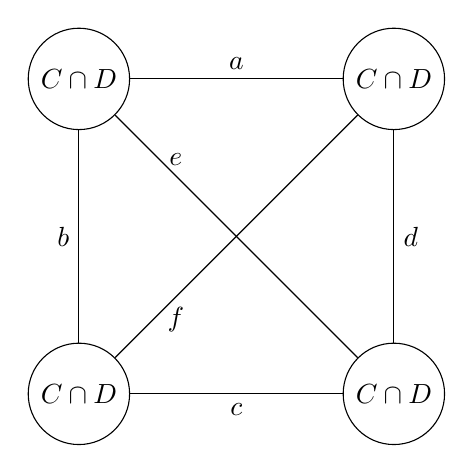
\begin{tikzpicture}
    \node[shape=circle,draw=black] (A) at (0,4) {\(C \cap D\)};
    \node[shape=circle,draw=black] (B) at (4,4) {\(\stcomp{C} \cap D\)};
    \node[shape=circle,draw=black] (C) at (4,0) {\(\stcomp{C} \cap \stcomp{D}\)};
    \node[shape=circle,draw=black] (D) at (0,0) {\(C \cap \stcomp{D}\)};
    
    \path (A) edge node [above] {\(a\)} (B);
    \path (A) edge node [near start, above] {\(e\)} (C);
    \path (A) edge node [left] {\(b\)} (D);
    \path (B) edge node [right] {\(d\)} (C);
    \path (B) edge node [near end, below] {\(f\)} (D);
    \path (C) edge node [below] {\(c\)} (D);
    \end{tikzpicture}
    \caption{The four cuts and their all possible edge boundaries between them. Diagram taken from \cite[p.~4]{Kr90}.}
    \label{fig:cuts}
    \end{figure}

    Let 
    \begin{align*}
        a &= |\partial(C \cap D, \stcomp{C} \cap D)|, & d &= |\partial(\stcomp{C} \cap D, \stcomp{C} \cap \stcomp{D})|, \\
        b &= |\partial(C \cap D, C \cap \stcomp{D})|, & e &= |\partial(C \cap D, \stcomp{C} \cap \stcomp{D})|, \\
        c &= |\partial(C \cap \stcomp{D}, \stcomp{C} \cap \stcomp{D})|, & f &= |\partial(C \cap \stcomp{D}, \stcomp{C} \cap D)|.
    \end{align*}

    Then, 

    \begin{align*}
    \kappa &= |\partial(C)| \\
           &= |\partial(C, \stcomp{C})| \\
           &= |\partial(C, \stcomp{C} \cap D)| + |\partial(C, \stcomp{C} \cap \stcomp{D})| \\
           &= |\partial(C \cap D, \stcomp{C} \cap D)| + |\partial(C \cap \stcomp{D}, \stcomp{C} \cap D)| \\
           &\quad + |\partial(C \cap D, \stcomp{C} \cap \stcomp{D})| + |\partial(C \cap \stcomp{D}, \stcomp{C} \cap \stcomp{D})| \\
           &= a + f + e + c. && \text{(1)} \\
    \intertext{This corresponds exactly to the edges in the diagram emanating from \(C \cap D\) and \(C \cap \stcomp{D}\). Similarly,}
    \kappa &= |\partial(D)| = b + f + e + d. && \text{(2)} 
    \intertext{By (1) and (2),}
        2\kappa &= a + b + c + d + 2e + 2f. && \text{(3)} 
    \intertext{The sets \(C \cap D\) and \(\stcomp{C} \cap \stcomp{D}\) contain an end, %go over this part
    so \(\partial(C \cap D) = a + e + b \geq \kappa\) and \(\partial(\stcomp{C} \cap \stcomp{D}) = c+e+d \geq \kappa\). It follows that the sum \(a+b+c+d+2e \geq 2\kappa\). By comparison with (3), we have that \(f = 0\). Finally,}
    \kappa &= a + e + b = c + e + d.
    \intertext{Therefore, \(\partial(C \cap D)\) and \(\partial(\stcomp{C} \cap \stcomp{D})\) are minimal as required.} \altqedhere
\end{align*} 
\end{proof}

\subsubsection{Building structure trees}
Our goal in this section is to shed light on how to construct \emph{structure trees}, as in \cite{K10} and \cite{D13}. In particular, we are interested in the action of finitely generated groups with more than one end on structure trees of their Cayley graphs, and how this ties in with our aim of proving Stallings' theorem. As the construction is very detailed, we focus instead on providing some intuition without going into detail about the proofs.

To start, note that if \(\Gamma\) is the Cayley graph of a group \(G\) with respect to some finite generating set \(S \subseteq G\), then \(\Gamma\) is connected and the action of \(G\) on \(\Gamma\) is transitive (there is only one orbit of vertices).

\begin{definition}
    Cuts of vertices \(C, D \subset V(\Gamma)\) are \emph{nested} if one of the following conditions hold:
    \begin{enumerate}
        \item \(C \subset D\)
        \item \(D \subset C\)
        \item \(C \cap D = \varnothing\)
        \item \(C \cup D = V(\Gamma)\).
    \end{enumerate}
    Alternatively, cuts are nested if there is one empty corner. Cuts \(C,D\) are said to be \emph{non-nested} if they are not nested.
\end{definition}

Structure trees are trees which are constructed from \emph{structure cuts}, which are cuts \(C\) such that for any automorphism \(g \in \mathrm{Aut}(\Gamma)\), \(C\) and \(g(C)\) are nested. Let \(\mathcal{C} := \{g(C) \mid g \in \mathrm{Aut}(\Gamma)\}\) be this collection of cuts. If \(G\) acts on its Cayley graph \(\Gamma\), and if \(\mathcal{C}\) is a \(G\)-invariant set of nested cuts, then the action of \(G\) on \(\Gamma\) induces an action of \(G\) on a subset of the elements of \(\mathcal{C}\), which are called \(\mathcal{C}\)-blocks. From these \(\mathcal{C}\)-blocks, we can construct a tree --- in which \(\mathcal{C}\)-blocks form the vertices and edges are given by intersecting pairs of \(\mathcal{C}\)-blocks. The resulting tree is denoted \(T(\mathcal{C})\) and is called the \emph{structure tree}. If the action is transitive on \(\Gamma\), then it is also transitive on \(T(\mathcal{C})\).

Now that we have a transitive action on a infinite tree, Kr\"{o}n uses Bass-Serre theory to deduce that the group \(G\) splits over the stabiliser of an edge. As the action of a tree on its Cayley graph is free, there is some work to be done to show that the edge stabilisers of \(T(\mathcal{C})\) are finite.
In summary, this points to the following theorem:

\begin{theorem}[Opposite direction to Theorem~\ref{backimp}]
    Let \(G\) be an infinite finitely generated group with more than one end. Then, \(G\) splits over some finite subgroup \(H\). 
\end{theorem}

\begin{remark}
    There are many further details which have been omitted from the explanation above: for example, how do we define \(\mathcal{C}\)-blocks and how exactly does the action of \(G\) on its Cayley graph induce an action on these blocks? We will not address these in full, but instead will draw upon an example taken from \cite[p.~14]{D13}.
\end{remark}

\begin{figure}[h!]
    \centering
    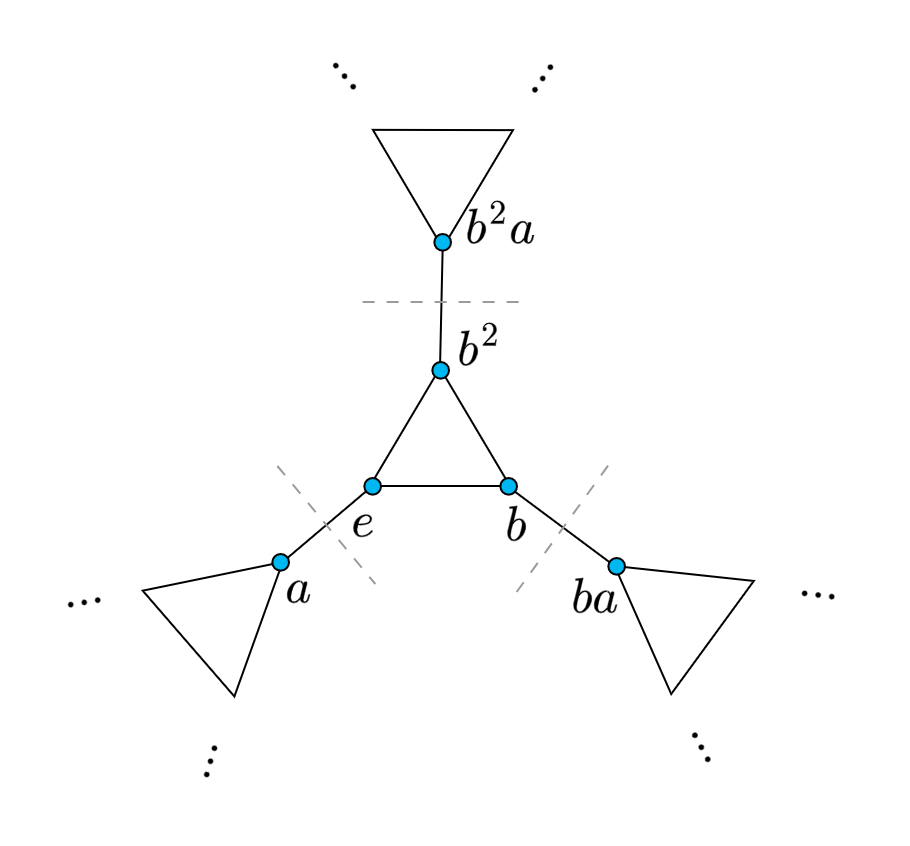
\includegraphics[width=0.6\linewidth]{sections/talia/CayleyGraph.png}
    \caption{A Cayley graph for \(\mathrm{PSL}(2,\mathbb{Z})\) with generating set \(\{a,b,a^{-1},b^{-1}\}\). The cuts are shown by dotted lines, and blue vertices form the block corresponding to this set of cuts.}
    \label{fig:psl}
\end{figure}

\begin{example}[Blocks in a Cayley graph for \(\mathrm{PSL}(2,\mathbb{Z})\)]
    
    Here, we use without proof that 
    \[
    \mathrm{PSL}(2,\mathbb{Z}) \cong \mathbb{Z}/2\mathbb{Z} * \mathbb{Z}/3\mathbb{Z} = \langle a,b \mid a^2 = b^3 =1 \rangle.
    \]
    Let the Cayley graph of \(\mathrm{PSL}(2,\mathbb{Z})\) generated by \(a, b\) and their inverses be called \(\Gamma\).
    Consider the three cuts denoted by the dotted lines in Figure~\ref{fig:psl}. The vertices in each cut lie in each of the three connected components which extend outwards toward infinity from each of the three dotted lines respectively. These three cuts form a set \(\mathcal{C}\), and the block relative to this \(\mathcal{C}\) is given by the blue vertices.
\end{example}

\begin{comment}
\subsubsection{Nested cuts}
\textcolor{cyan}{I don't really like this section. I feel like I can follow the individual theorems but I don't really understand what this part of the paper is trying to say. I'm going to try to replace this.}
Our goal in this section is to briefly explore how to construct \emph{structure trees}. In particular, we are interested in the action of finitely generated groups with more than one end on structure trees of their Cayley graphs. In order to build these trees, we introduce what is means for cuts to be \emph{nested}. Several results in this section are stated without proof, however proofs can be found in \cite[Chapter~3]{K10}. 

Recall the four cuts \(C \cap D, \stcomp{C} \cap D, C \cap \stcomp{D}, \stcomp{C} \cap \stcomp{D}\) which we referred to as \emph{corners} of \(C\) and \(D\). We say that the cuts which lie on diagonal corners of the diagram in Figure~\ref{fig:cuts} are \emph{opposite}.

\begin{definition}[Nested]
    Cuts of vertices \(C, D \subset V(\Gamma)\) are \emph{nested} if one of the following conditions hold:
    \begin{enumerate}
        \item \(C \subset D\)
        \item \(D \subset C\)
        \item \(C \cap D = \varnothing\)
        \item \(C \cup D = V(\Gamma)\).
    \end{enumerate}
    Alternatively, cuts are nested if there is one empty corner. Cuts \(C,D\) are said to be \emph{non-nested} if they are not nested.
\end{definition}

\begin{lemma}
    Let \(C, D, E\) be cuts of vertices and let \(C\) and \(D\) be non-nested. 
    \begin{enumerate}[(i)]
    \item If \(E\) is non-nested with two opposite corners of \(C\) and \(D\), then \(E\) is non-nested with both \(C\) and \(D\). 
    \item If \(E\) is non-nested with some corner of \(C\) and \(D\), then \(E\) is either non-nested with \(C\) or non-nested with \(D\).
    \end{enumerate}
\end{lemma}

\begin{remark}
  Note that this theorem does not hold when \(C,D,E\) are arbitrary sets of vertices instead of cuts.  
\end{remark}

\begin{example}
    Let \(\Gamma\) be the Cayley graph of \(F_2\) with generating set \(\{a,b,a^{-1},b^{-1}\}\). Let \(C\) be the ray given by \(\{e,a,a^2,a^3, \dots\}\), \(D = \{e, b, b^2, b^3 \dots\}\) and \(E = \{e, a, ab, aba,  \dots\}\). The sets \(C, D\) are non-nested. The corners of \(C\) and \(D\) are the following.
    \begin{align*}
        C \cap D & = \{e\} \\
        \stcomp{C} \cap D & = \{b,b^2,b^3,\dots\} \\
        C \cap \stcomp{D} & = \{a,a^2,a^3, \dots\} \\
        \stcomp{C} \cap \stcomp{D} & = \langle a,b \rangle \setminus \left\{ \langle a \rangle \cup \langle b \rangle \right\}
    \end{align*}
    The vertex set \(E\) is non-nested with the first corner, but non-nested with the others. By (i), we expect that \(E\) is non-nested with \(C\) and with \(D\), and one can verify that this is the case.
\end{example}

\begin{definition}[Minimal non-nested cuts]
    Let \(C\) be a cut and let \(M(C)\) be the set of minimal cuts which are non-nested with \(C\). Let \(m(C) = |M(C)|\) be the cardinality of this set. 
\end{definition}

\begin{lemma}
\label{lem:ineq}
    Let \(C\) and \(D\) be non-nested cuts and suppose \(C \cap D\) and \(\stcomp{C} \cap \stcomp{D}\) are cuts. Then,
    \[
        m(C \cap D) + m(\stcomp{C} \cap \stcomp{D}) < m(C) + m(D).
    \]
\end{lemma}

\begin{definition}
    Let \(\mathcal{C}\) be the set of all minimal cuts. Set \(m = \min\{m(C) \mid C \in \mathcal{C}\}\).  A minimal cut \(C\) with \(m(C) = m\) is called \emph{optimally nested}.
\end{definition}

\begin{theorem}
    Optimally nested cuts are nested with all other optimally nested cuts.
\end{theorem}

\begin{proof}
    \cite[Theorem~3.3, p.~5--6]{K10}
    Suppose there are optimally nested minimal cuts \(E\) and \(F\) which are non-nested. Then \(m \geq 1\). There cannot be two adjacent corners which do not contain an end, because \(C, D, \stcomp{C}\) and \(\stcomp{D}\) all contain an end (since they are cuts and must contain a ray by definition, and contain all equivalent rays by Proposition~\ref{prop:ray}). Hence there is a pair of opposite corners which contain an end. By relabeling, we can assume that these corners are \(C \cup D\) and \(\stcomp{C} \cap \stcomp{D}\) and by Lemma~\ref{lem:mincuts}, \(C \cap D\) and \(\stcomp{C} \cap \stcomp{D}\) are minimal cuts.
    Using Lemma~\ref{lem:ineq},
    \[
    m(C \cap D) + m(\stcomp{C} \cap \stcomp{D}) < m(C) + m(D) = 2m.
    \]
    Therefore, one of the summands on the left side is less than \(m\), contradicting the minimality of \(m\). 
\end{proof}

\textcolor{cyan}{Once I understand this I really want to reinforce why this theorem is important and why we care about nested cuts. Kron talks about G-invariant automorphisms and this feels important}

From these systems of nested cuts, one can build a tree known as the \emph{structure tree}. 

With a few more definitions, we conclude this section by illustrating this construction.

\begin{definition}[Boundary of a cut]
    Let \(C\) be a cut. The \emph{boundary} of \(C\), denoted by \(\Delta(C)\), is the set of vertices in \(\stcomp{C}\) which are adjacent to a vertex in \(C\).
\end{definition}

\begin{definition}[Blocks]
    Let \(\mathcal{C}\) be a set of cuts. A maximal set of vertices \(B\) for which the following condition is satisfied is called a \(\mathcal{C}\)-block. 
    The condition is as follows: for all \(C \in \mathcal{C}\), either \(B \subset C \cup \Delta(C)\) or \(B \subset \stcomp{C} \cup \stcomp{\Delta(C)}\).
\end{definition}

\begin{definition}[Nested set of cuts]
    A set of minimal cuts \(\mathcal{C}\) is \emph{nested} if any two cuts \(C, D \in \mathcal{C}\) are nested. 
\end{definition}

\begin{construction}[Structure tree]
\label{const:structuretree}
    Given a nested set \(\mathcal{C}\) of minimal cuts, we define a graph \(T = T(\mathcal{C})\).
    \begin{itemize}
        \item Take the vertex set \(V(T)\) to be the set of \(\mathcal{C}\)-blocks.
        \item Two vertices are adjacent if they intersect as \(\mathcal{C}\)-blocks.
    \end{itemize}
\end{construction}

\begin{lemma}
\cite[Theorem~4.2,p.~7]{K10}
    The structure tree defined in Construction~\ref{const:structuretree} is a tree.
\end{lemma}
\end{comment}

\subsection{Links to Bass--Serre theory and further questions}
\subsubsection{Generalisations}
Stallings' structure theorem in the language of Bass--Serre theory gives the following useful corollary. 
\begin{corollary}
    A finitely generated group with more than one end has a non-trivial action on a tree with finite edge stabilisers.
\end{corollary}

Furthermore, from Stallings' structure theorem we can derive an even stronger classification.
\begin{theorem}[Stalling's Structure Theorem II]
    Stallings' structure theorem (Theorem~\ref{thm:SST}) extends to the following classification: 
    \begin{itemize}
        \item (1) corresponds to the case in which \(G\) has exactly two ends,
        \item (2) corresponds to the case where \(G\) has infinitely many ends and is torsion-free, and
        \item (3) corresponds to the case where \(G\) has infinitely many ends and has torsion.
    \end{itemize}
\end{theorem}

It seems that there is no similar classification for one-ended groups. Since most finitely generated infinite groups are not virtually \(\mathbb{Z}\) and cannot be split over a finite subgroup, we can take away the conclusion that most infinite finitely generated groups are in fact one-ended.

\subsubsection{Further research}
There is plenty more to be explored here and we give two possible directions for further investigation. 

\textbf{1.} \textit{``If most finitely generated groups are one-ended, what are some other examples other than \(\mathbb{Z}^2\)?''} 

In particular, a large class of hyperbolic groups are one-ended:

\begin{theorem} \cite{S96}\label{wetotallyplannedthis}
    A hyperbolic group is one-ended if its Gromov boundary is a non-empty connected space.
\end{theorem}

Hence, a set of examples would be the surface groups \(\pi_1(\Sigma_g)\) for \(g \geq 2\). One could look into similar theorems for small cancellation, Fuschian, or right-angled Artin groups. We return to discuss a related result in Section 5 (c.f. Theorem~\ref{twinning}). 

\vspace{1em}
\textbf{2.} \textit{``Does there exist a notion of ends of a group for an infinitely generated group? Do Stallings' results generalise further in this direction?''}
The answer to both of these questions is yes. The definition of such an end and the theorem below is given in \cite{phdthesis} (originally \cite{D89}).

\begin{theorem}
     Let \(G\) be a group. The following are equivalent:
     \begin{enumerate}[(i)]
         \item \(e(G) > 1\).
         \item For any non-trivial free \(G\)-module \(M\), \(H^1(G,M) \neq 0\).
         \item There exists a tree on which \(G\) acts without global fixed points and finite edge stabilisers.
         \item One of the following holds:
         \begin{itemize}
             \item \(G\) splits as an amalgam over a finite subgroup \(H\),
             \item \(G\) splits as a HNN-extension over a finite subgroup \(H\),
             \item \(G\) is countably infinite and locally finite.
         \end{itemize}
         \item \(e(G) = 2\) or \(e(G) = \infty\).
     \end{enumerate}
\end{theorem}


% \printbibliography
\bibliographystyle{alpha}
\bibliography{bib/sean_refs,bib/alicja_refs,bib/lorna_refs,bib/talia_refs}

\end{document}
